\section{Teilversuch 4: Quantitative Vermessung des normalen Zeeman-Effekts (transversale Beobachtung)}
	Es gab am Anfang eine Überbeleuchtung:
	\begin{figure}[!ht]
		\vspace{-0.2em}
	    \centering
	    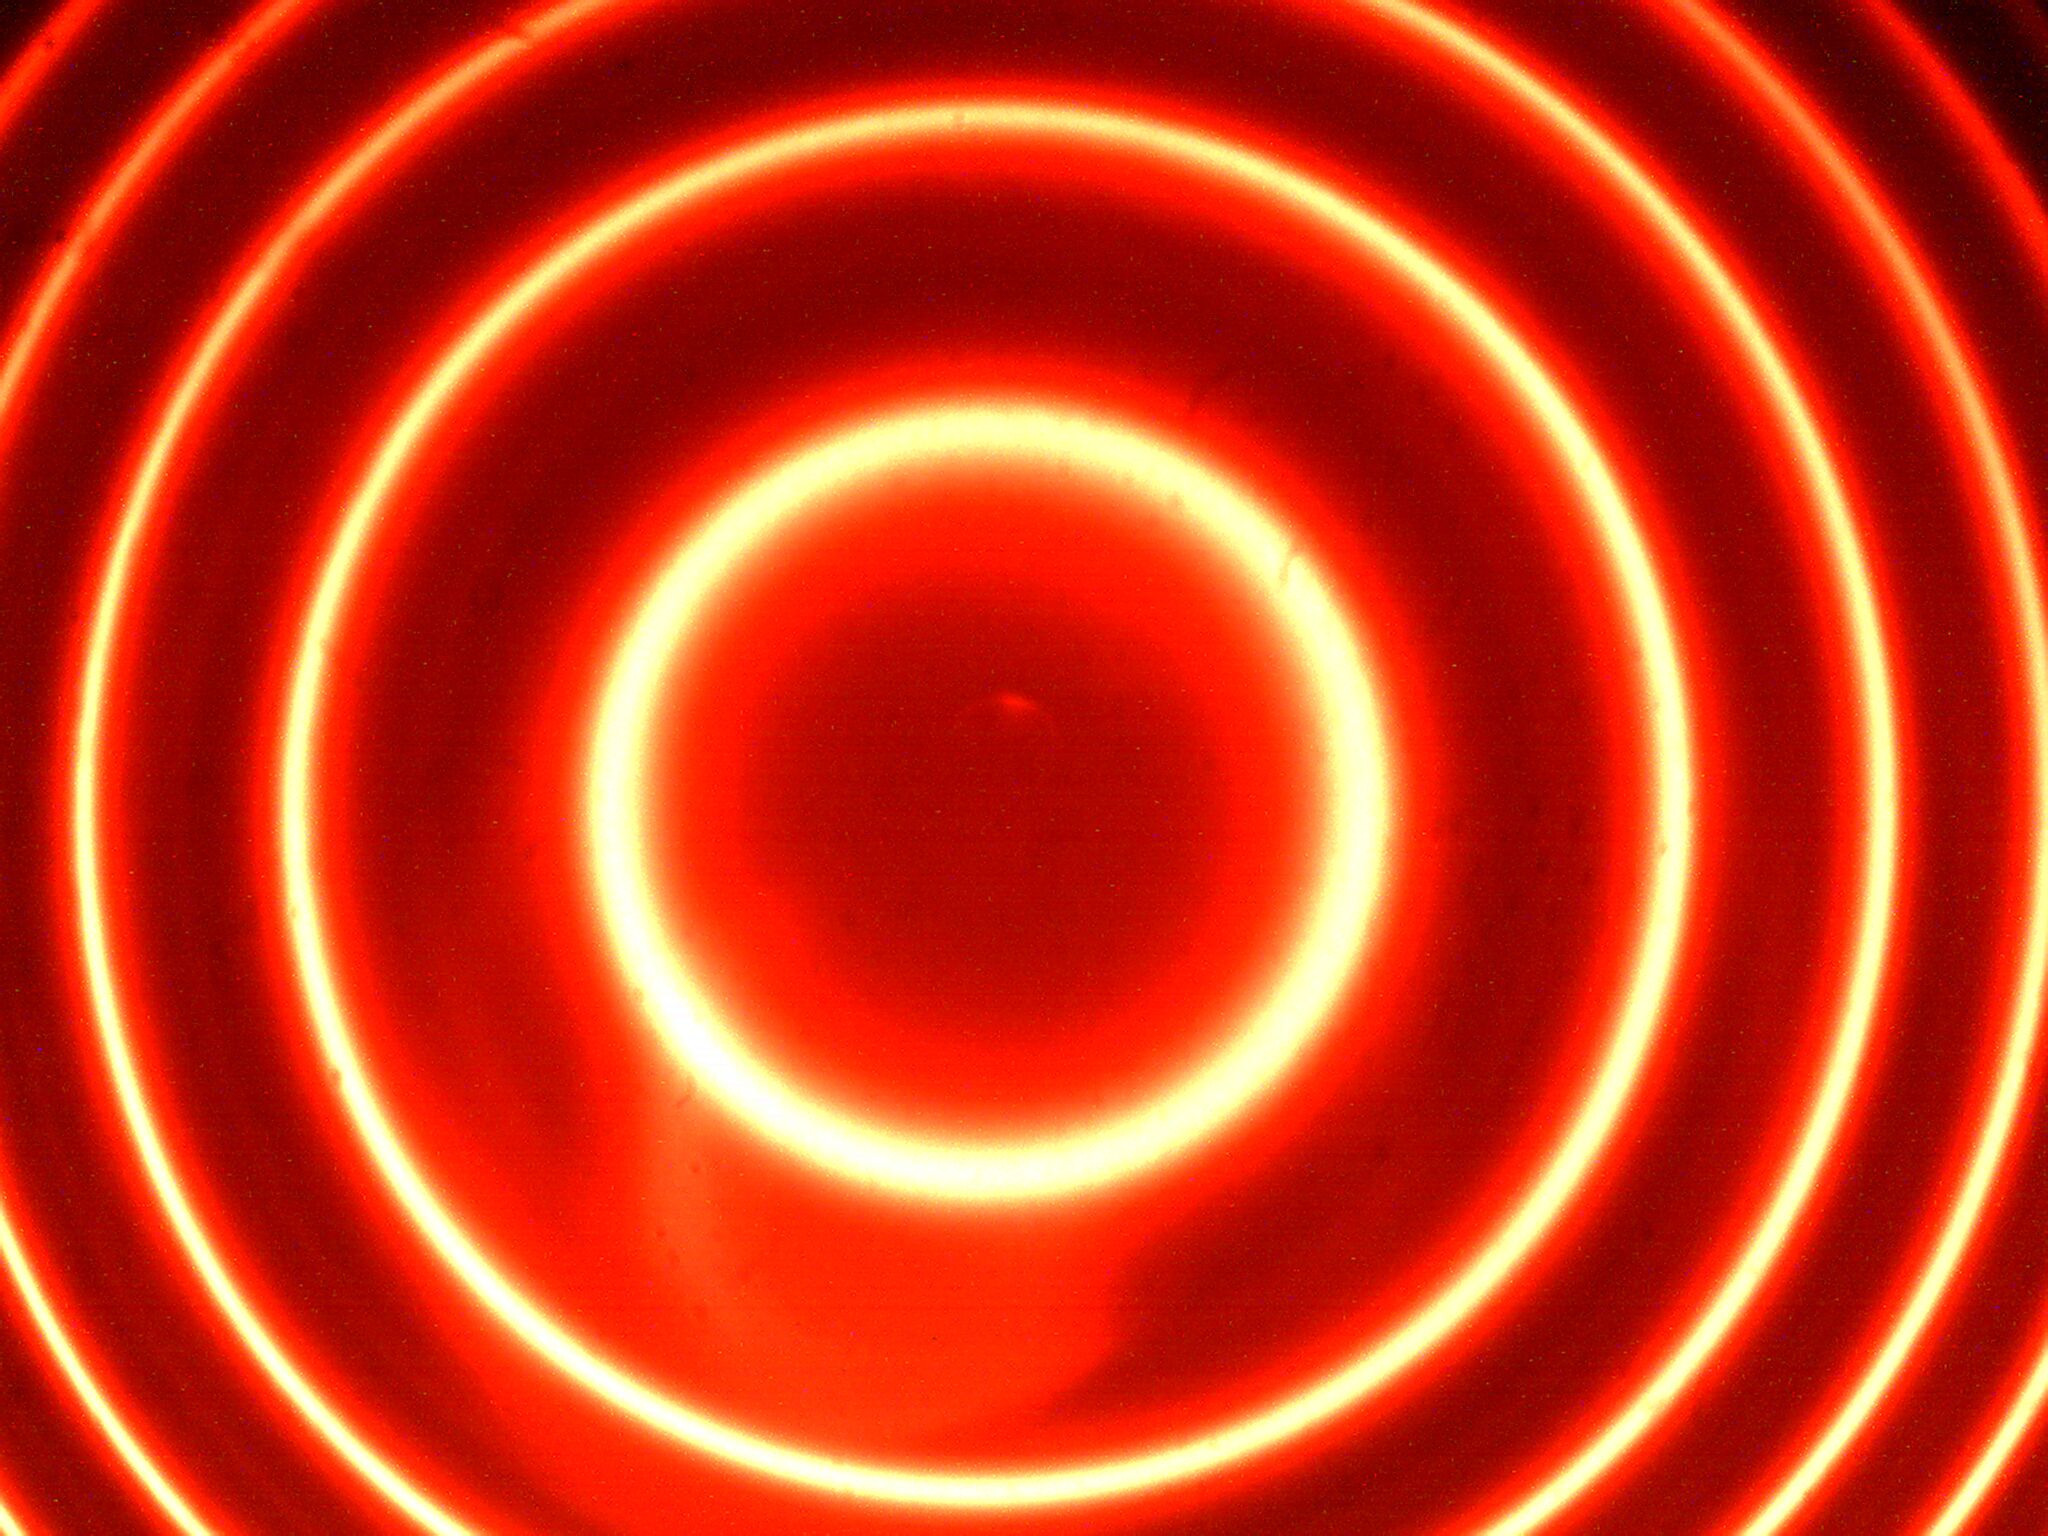
\includegraphics[width=0.55\textwidth]{images/Capture_810.bmp.jpg}
	    \caption{Überbeleuchtete Interferenzringe von rote Emissionslinie}
	    \label{fig:red-fringes}
	    \vspace{-1em}
	\end{figure}

	Nach Anpassung der Beleuchtung im Program.
	\begin{figure}[!ht]
	    \centering
	    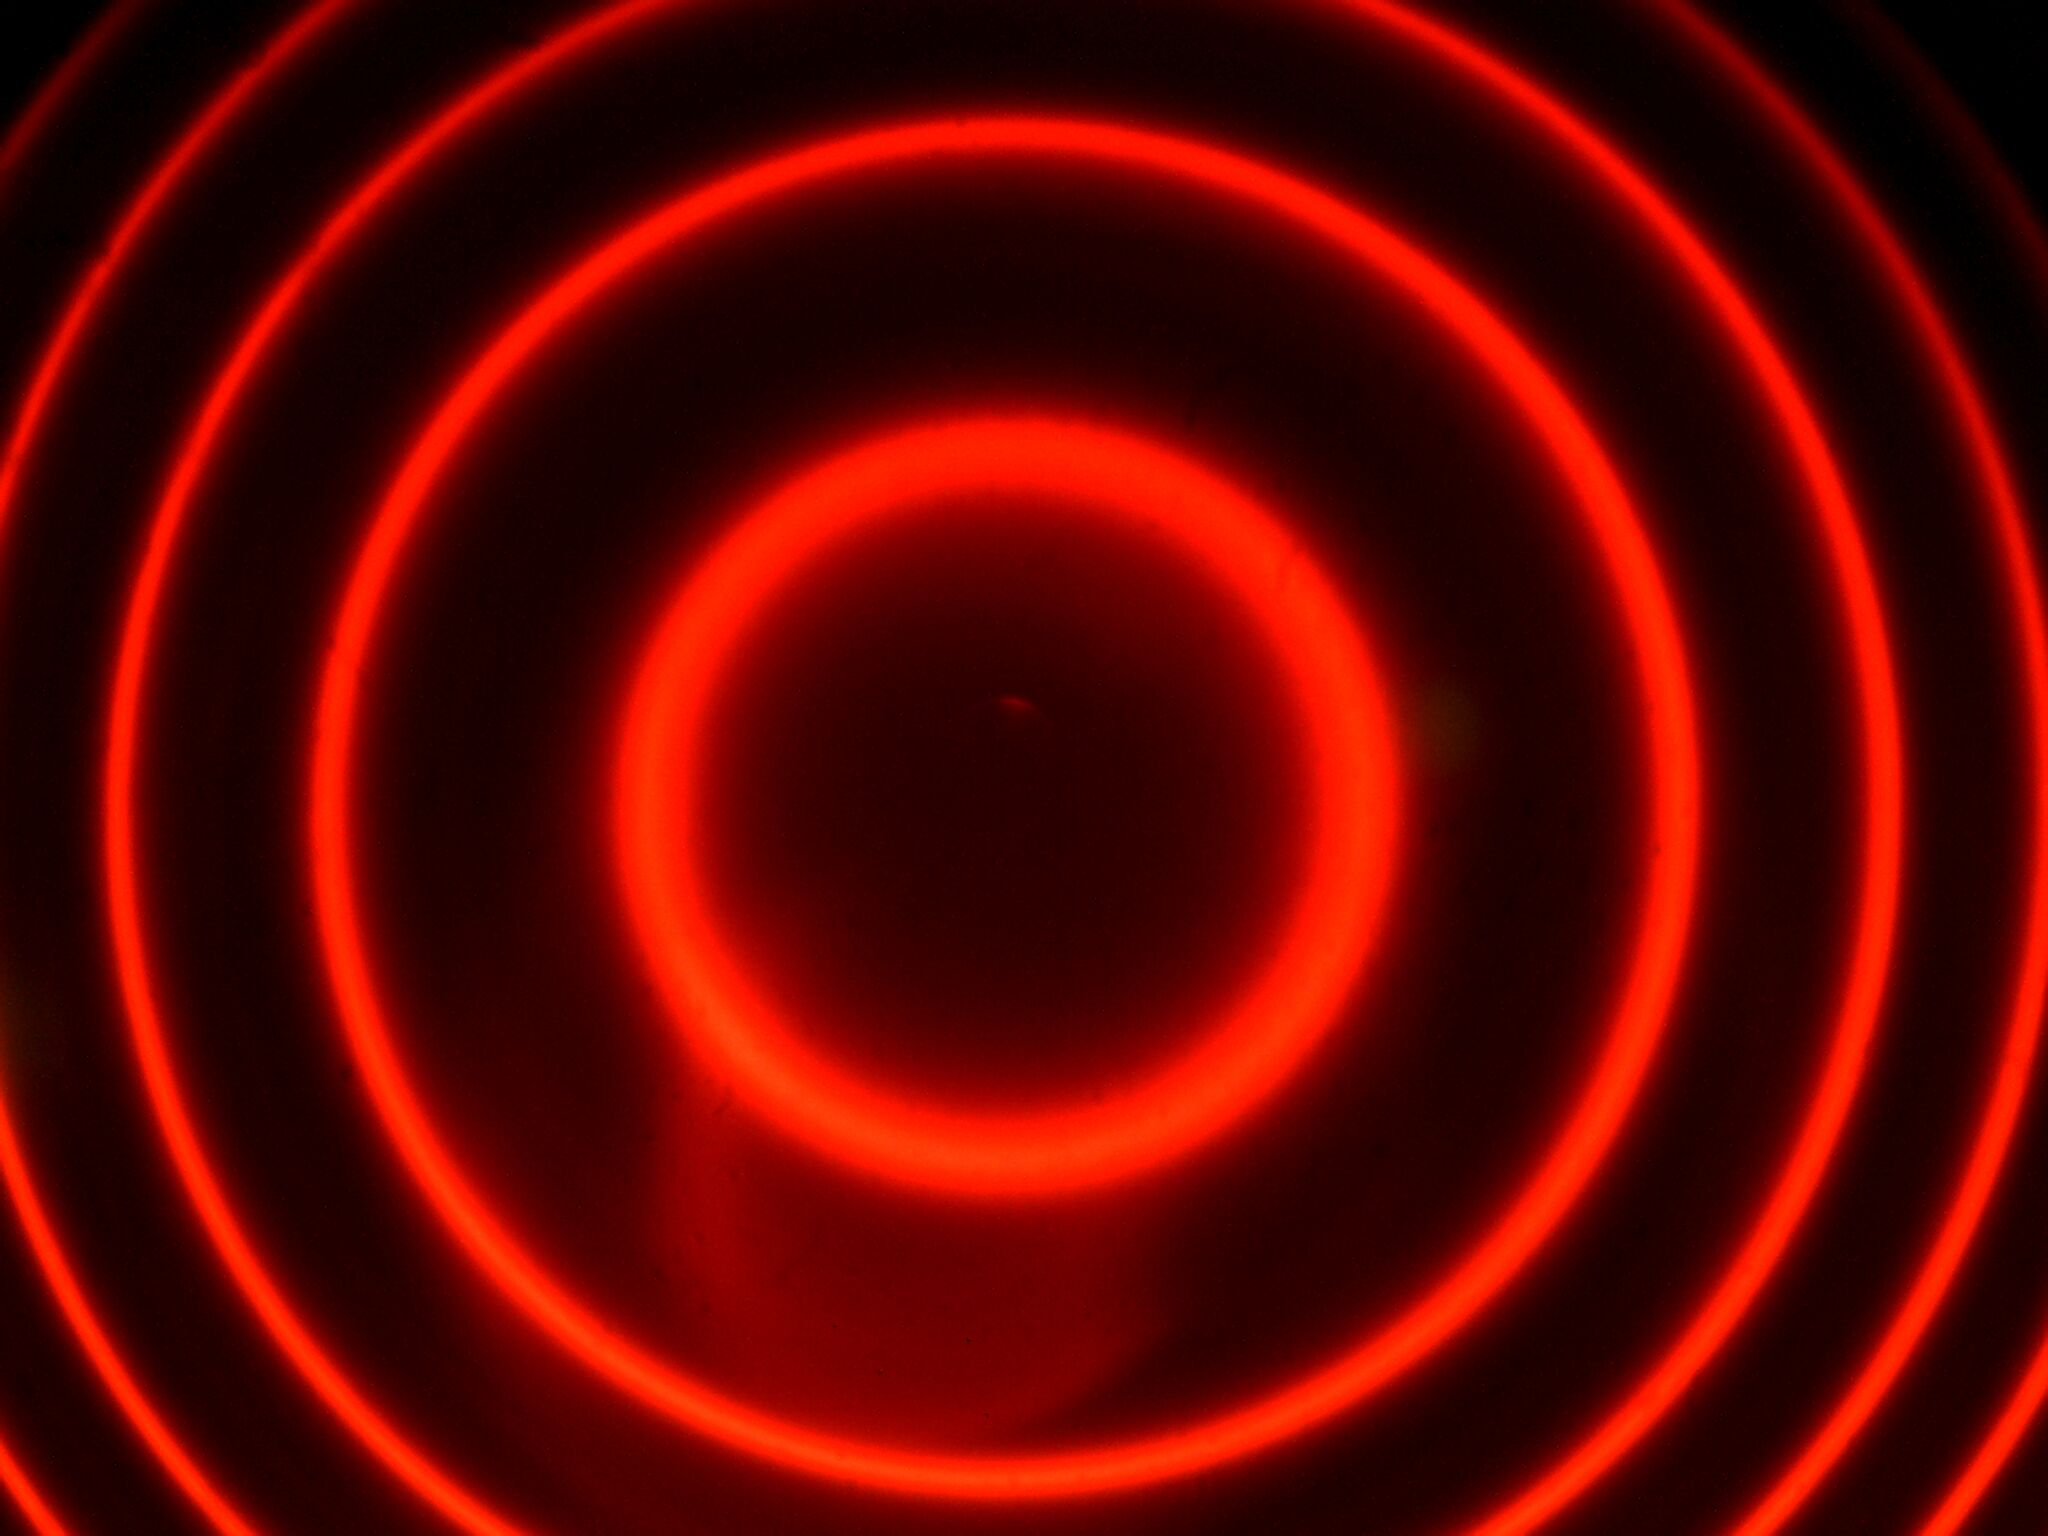
\includegraphics[width=0.45\textwidth]{images/Capture_811.bmp.jpg}
	    \hspace{1em}
	    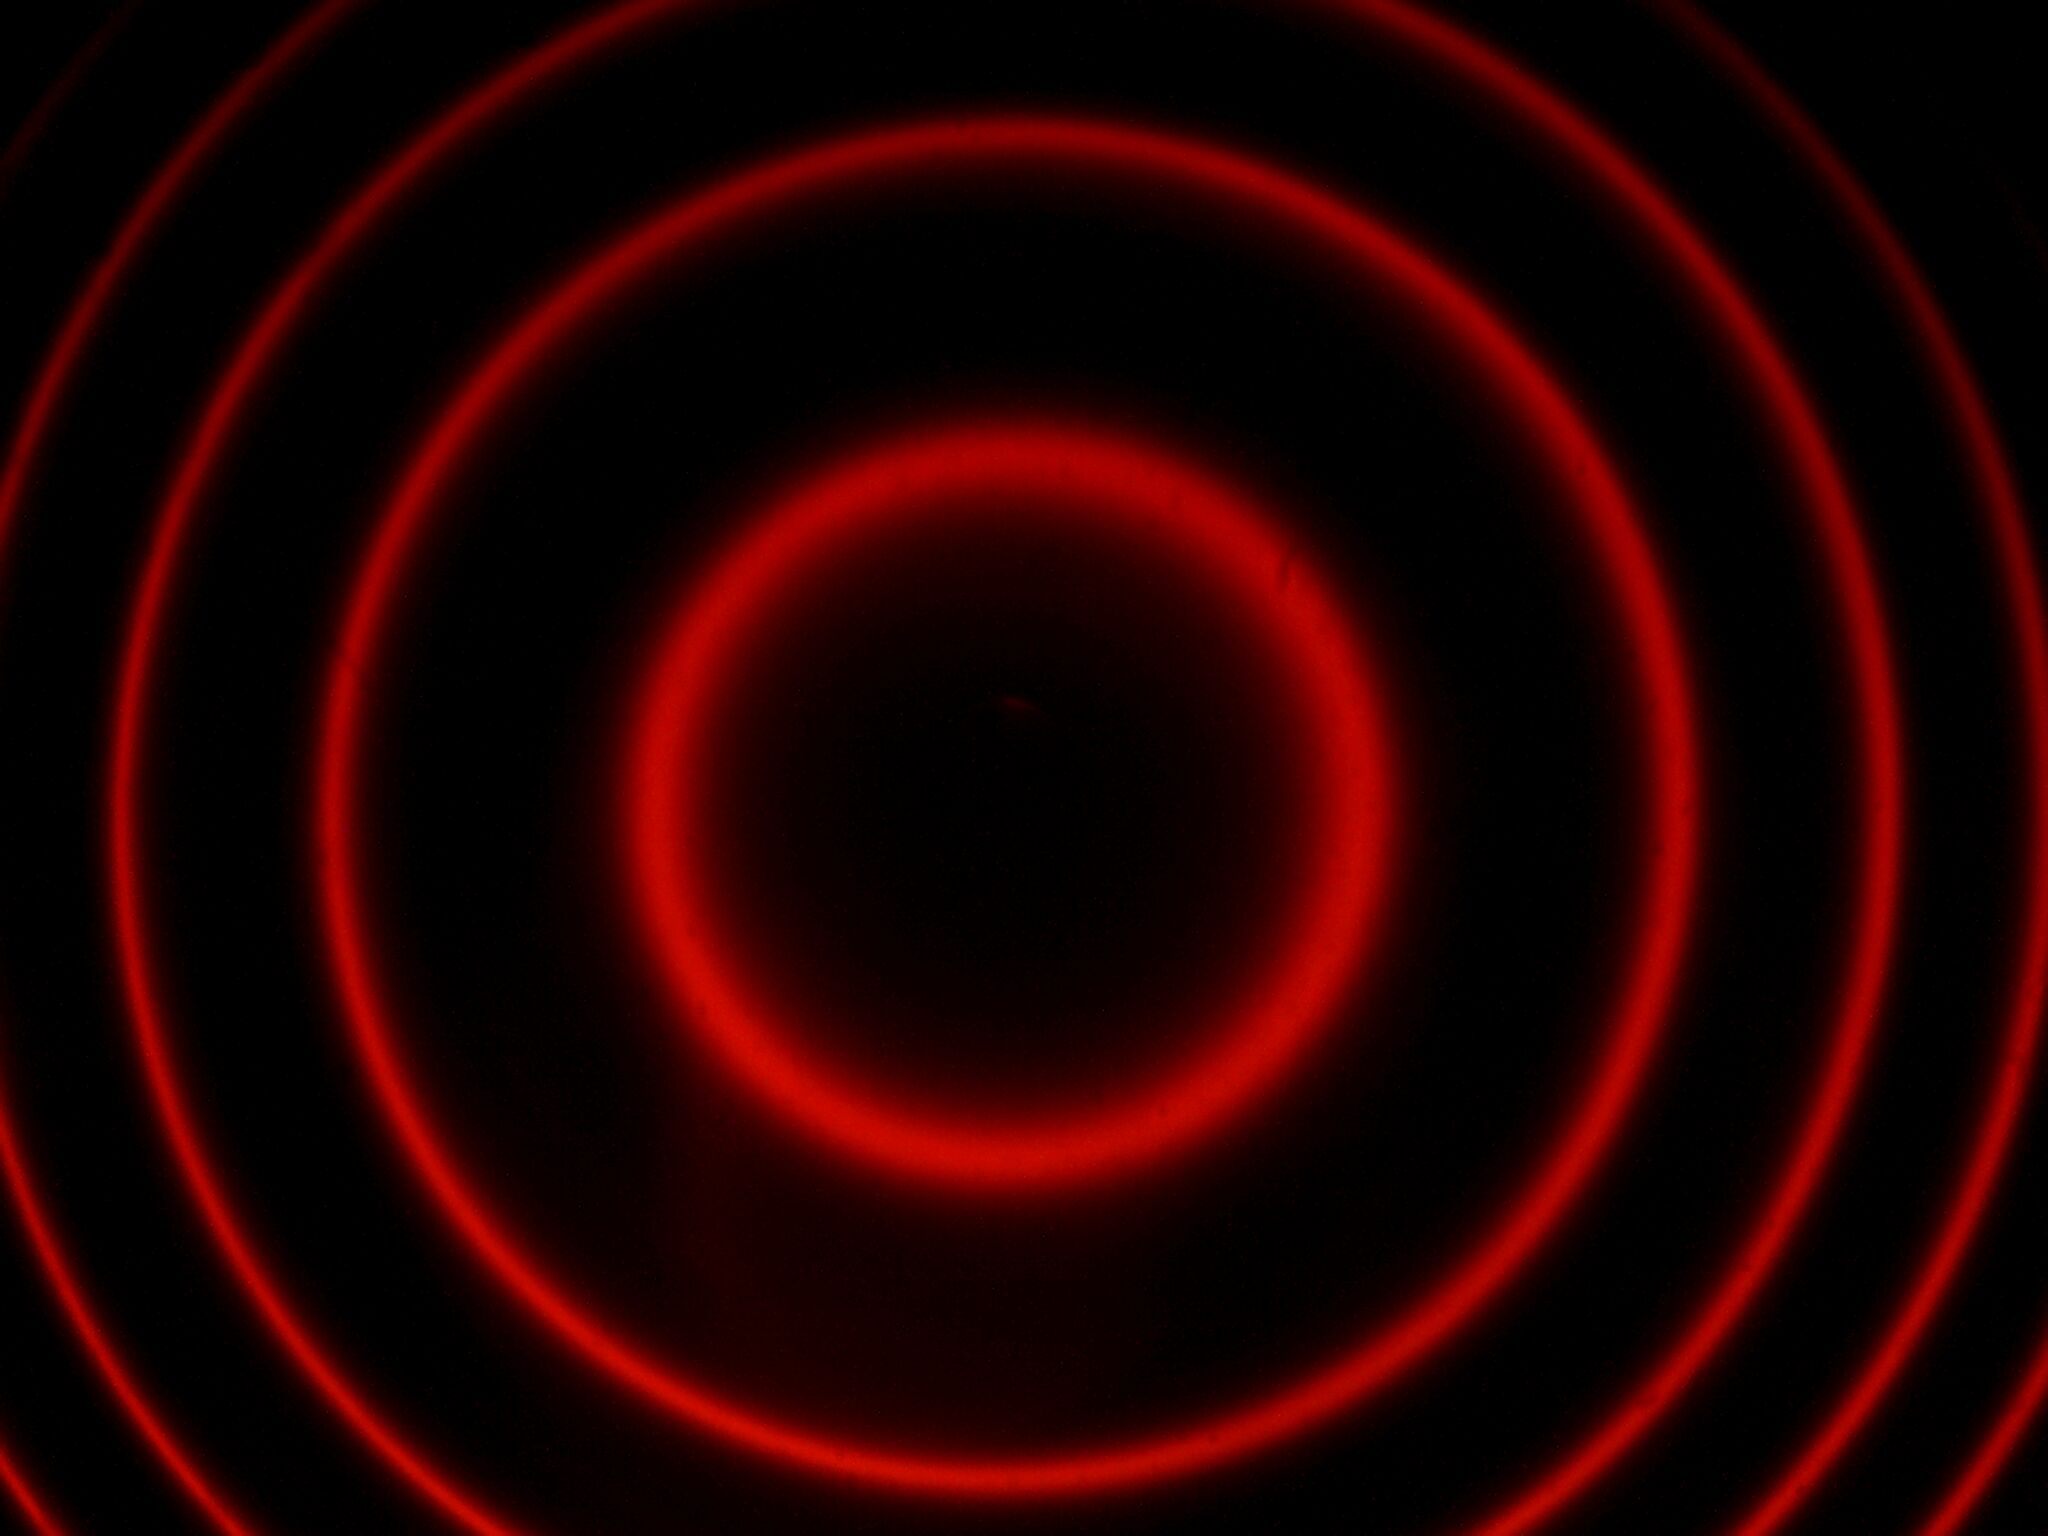
\includegraphics[width=0.45\textwidth]{images/Capture_812.bmp.jpg}
	    \caption{Interferenzringe von rote Emissionslinie. Ohne Polarisationsfilter (Links). Mit Polarisationsfilter (Rechts)}
	    \label{fig:red-fringes-pol}
	    \vspace{-0.5em}
	\end{figure}
	\begin{figure}[!ht]
	    \centering
	    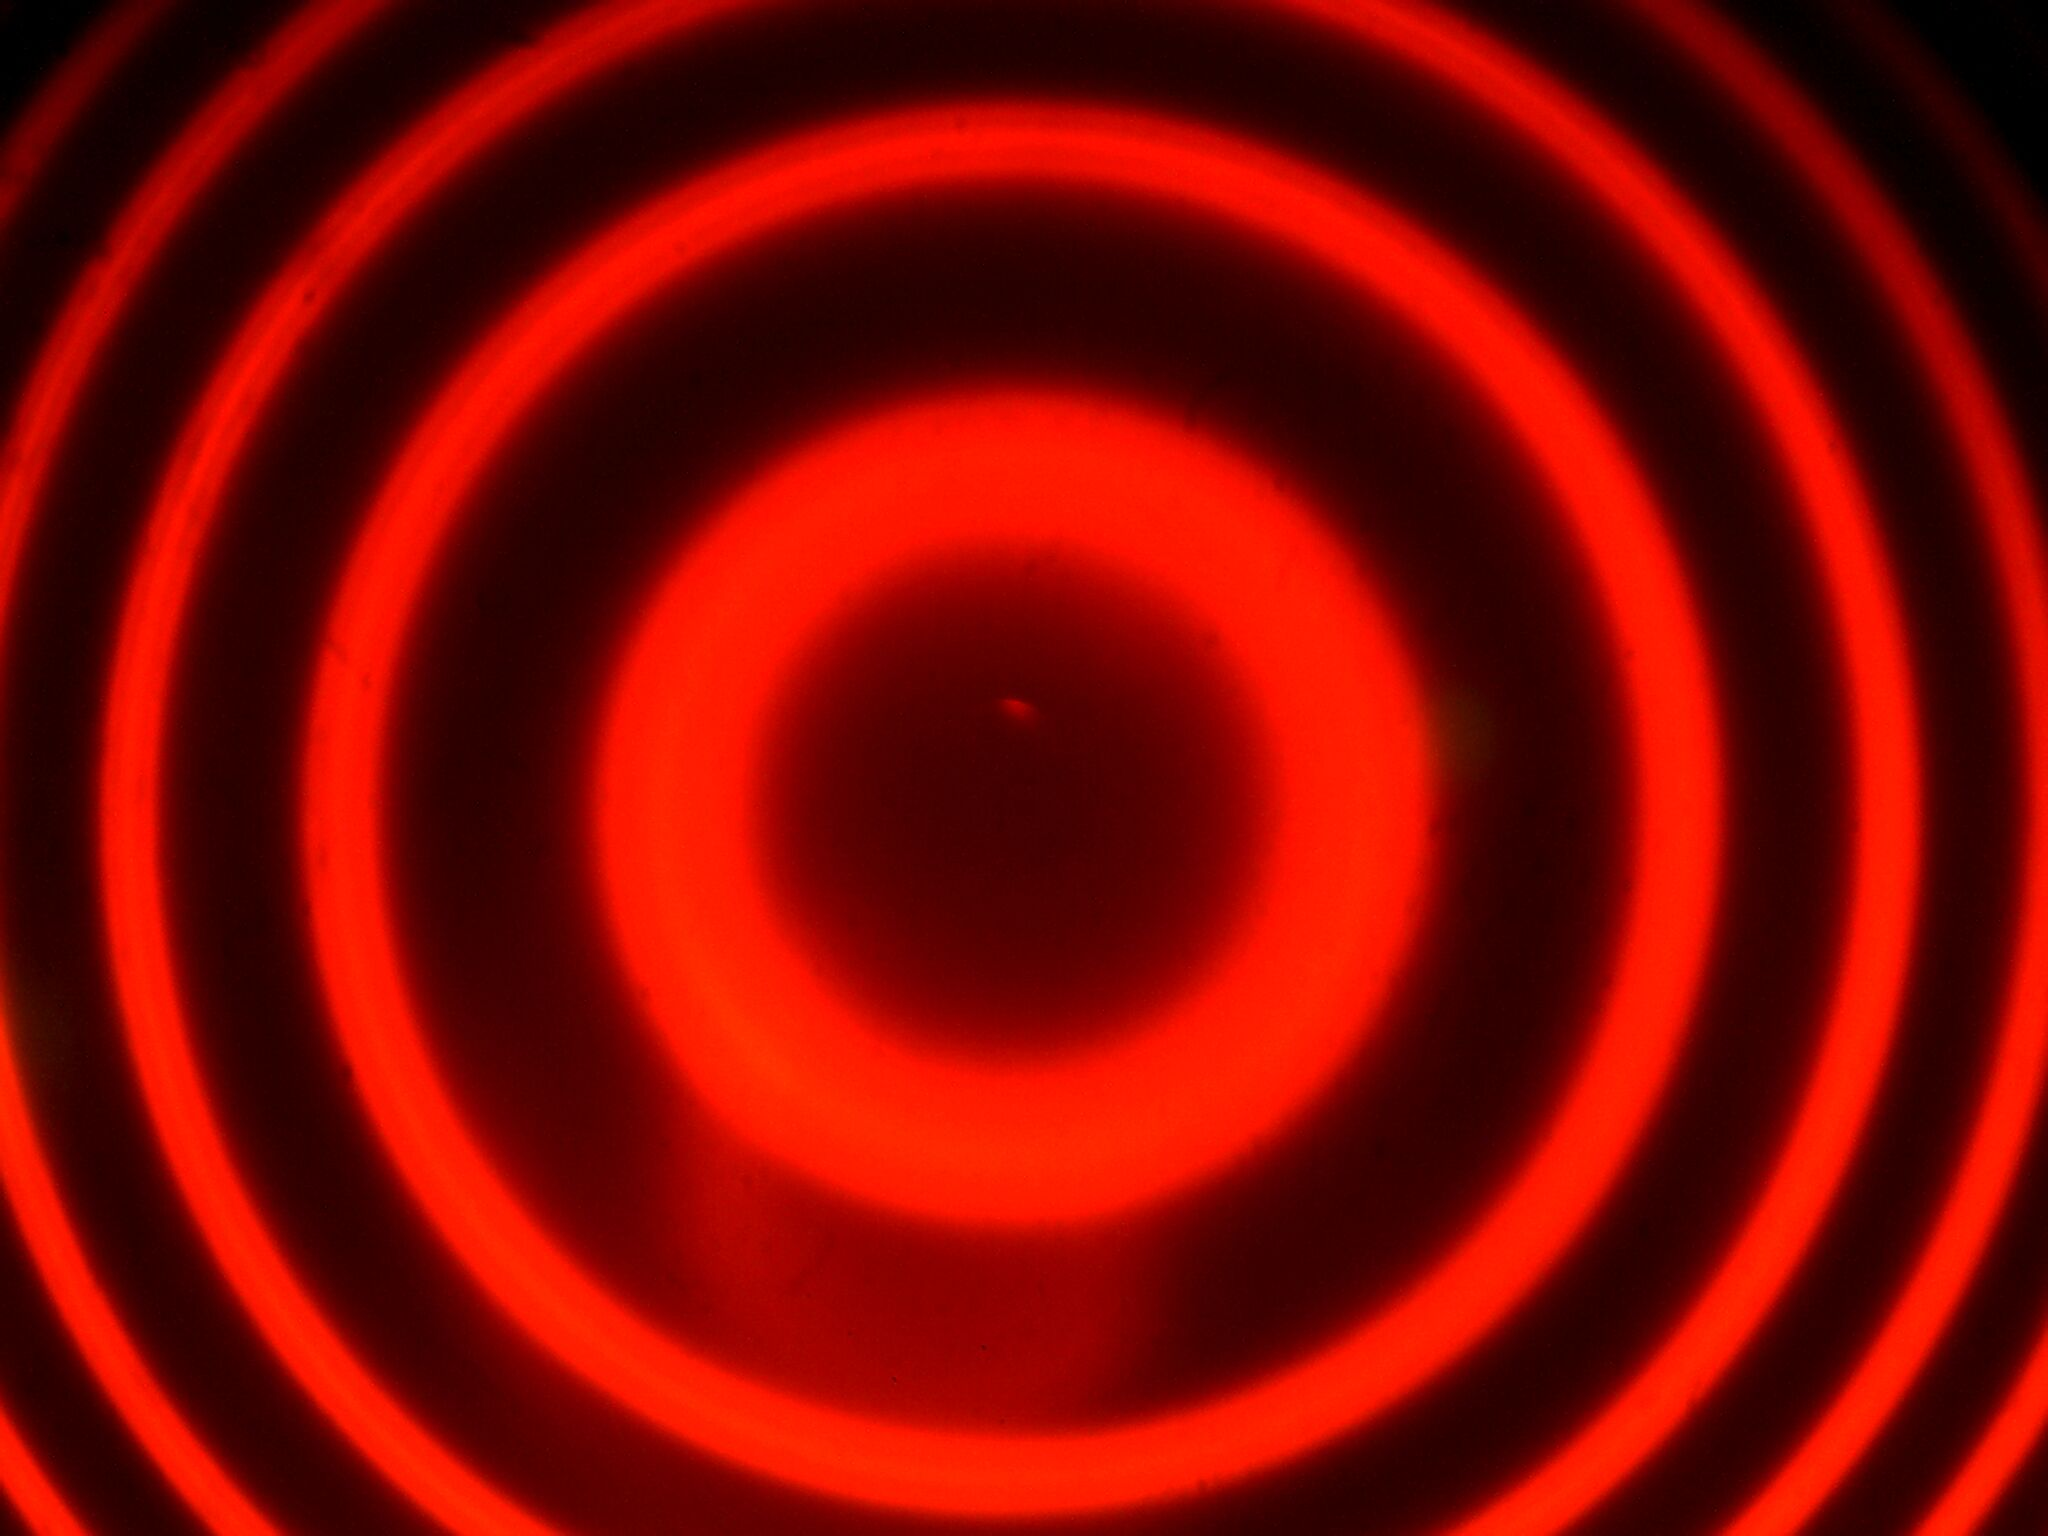
\includegraphics[width=0.45\textwidth]{images/Capture_814.bmp.jpg}
	    \hspace{1em}
	    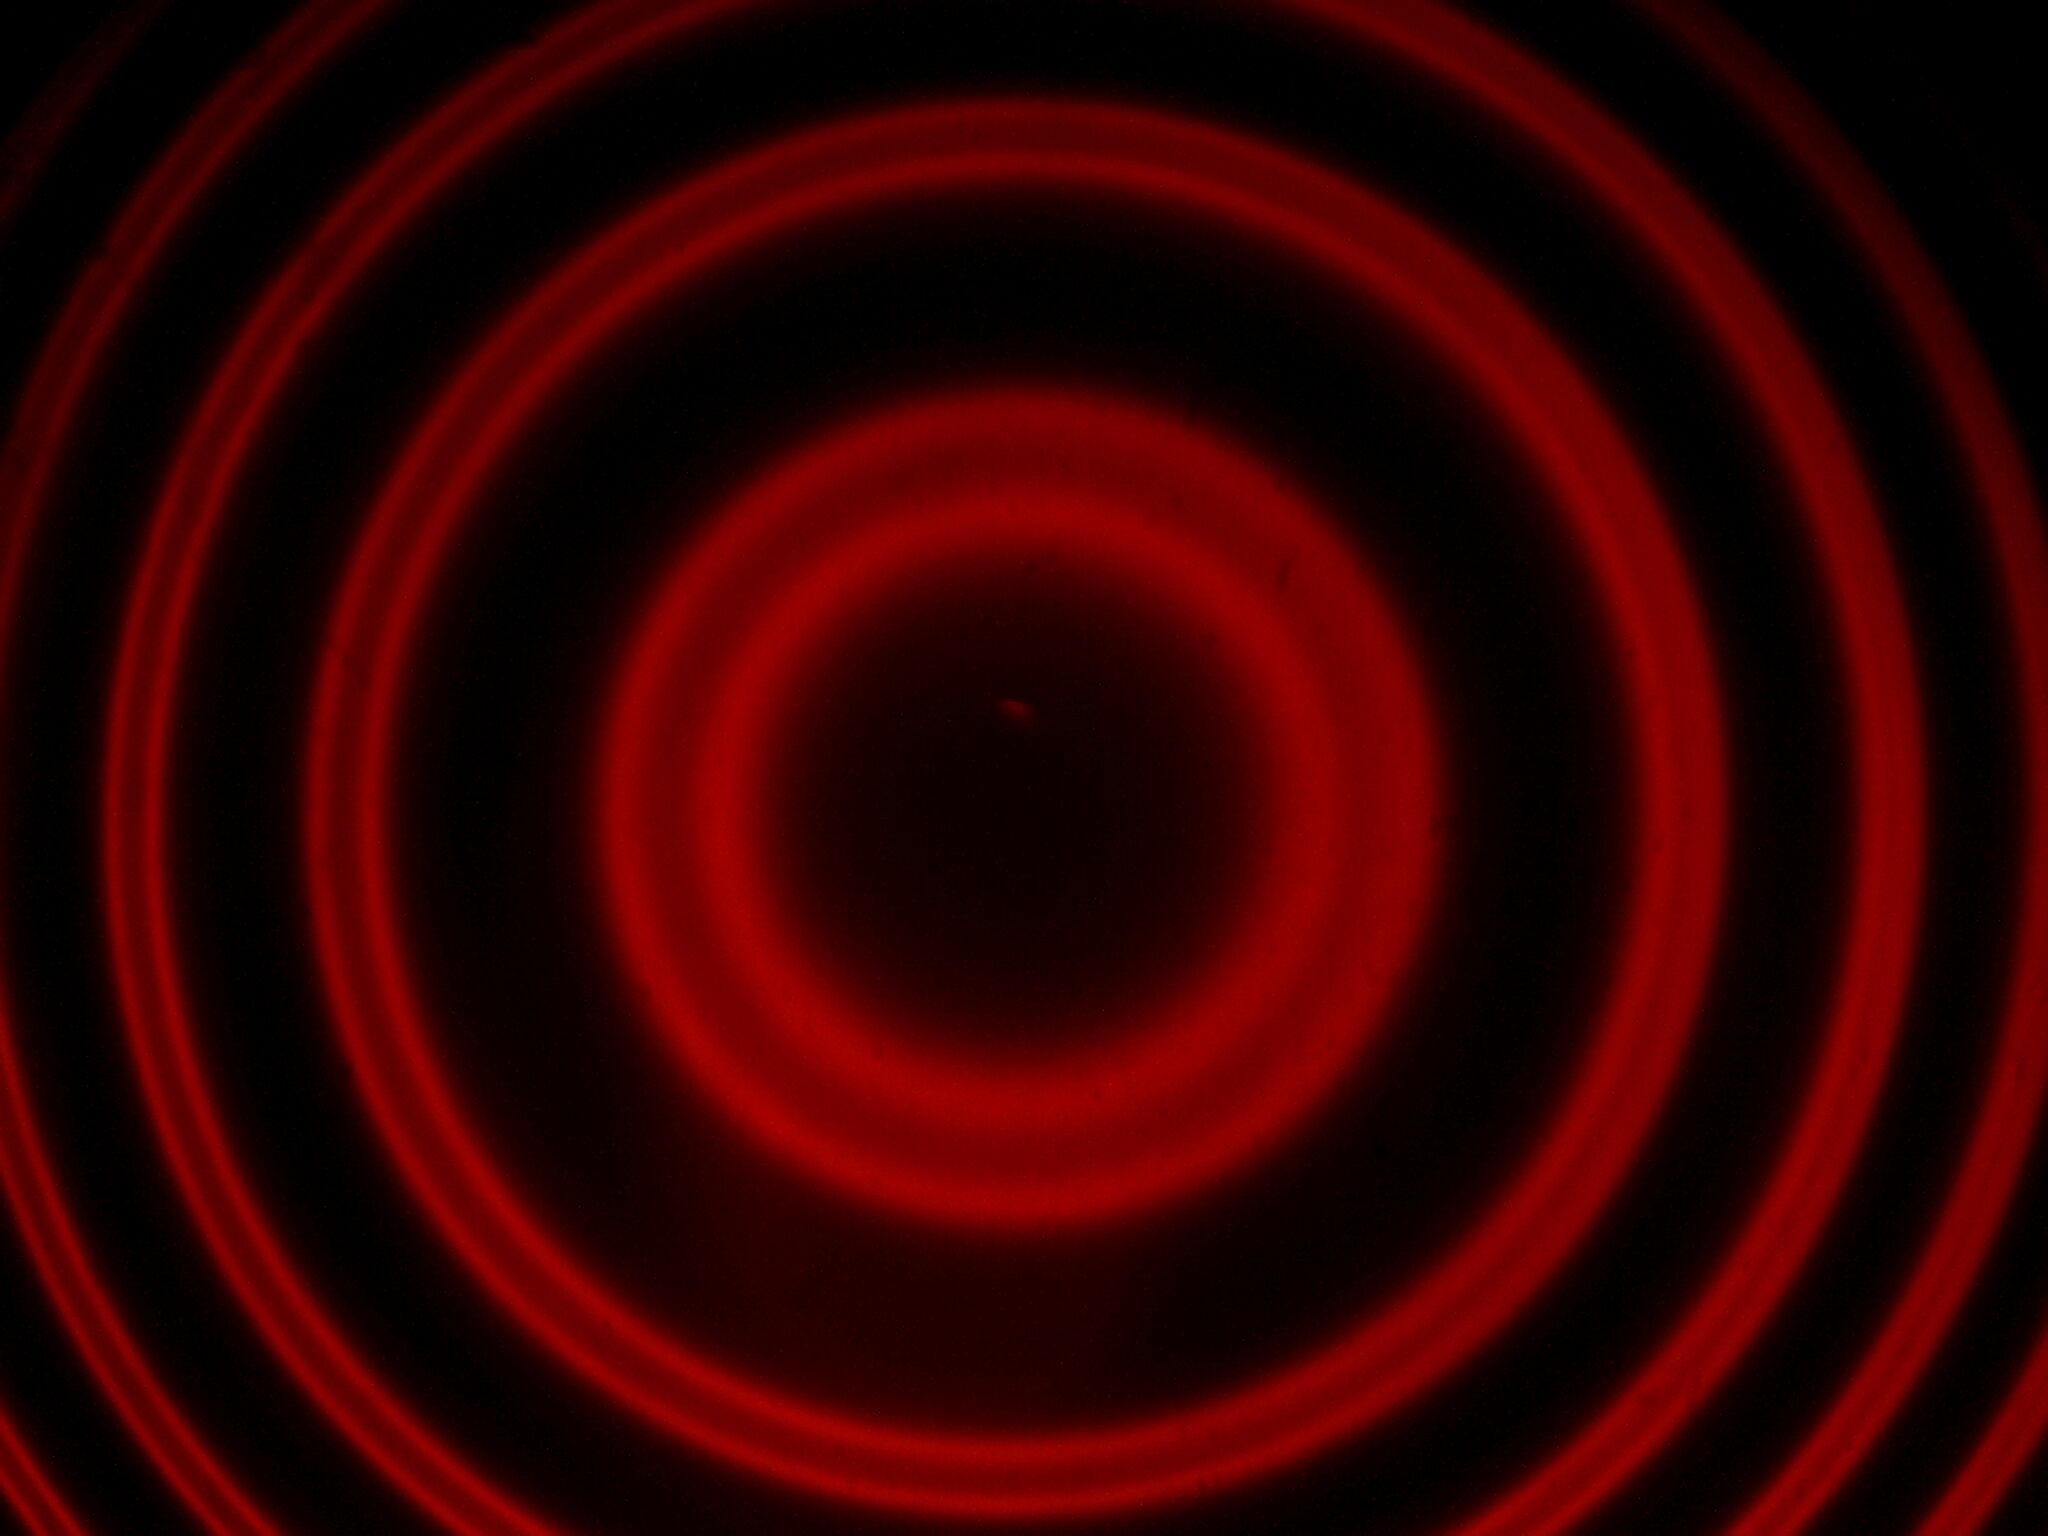
\includegraphics[width=0.45\textwidth]{images/Capture_813.bmp.jpg}
	    \caption{Interferenzringe von rote Emissionslinie im Magnetfeld $B \approx 2\text{ - }3 \si{\ampere}$. Ohne Polarisationsfilter (Links). Mit Polarisationsfilter (Rechts)}
	    \label{fig:red-fringes-pol-B}
	    \vspace{-0.5em}
	\end{figure}
	\begin{figure}[!ht]
	    \centering
	    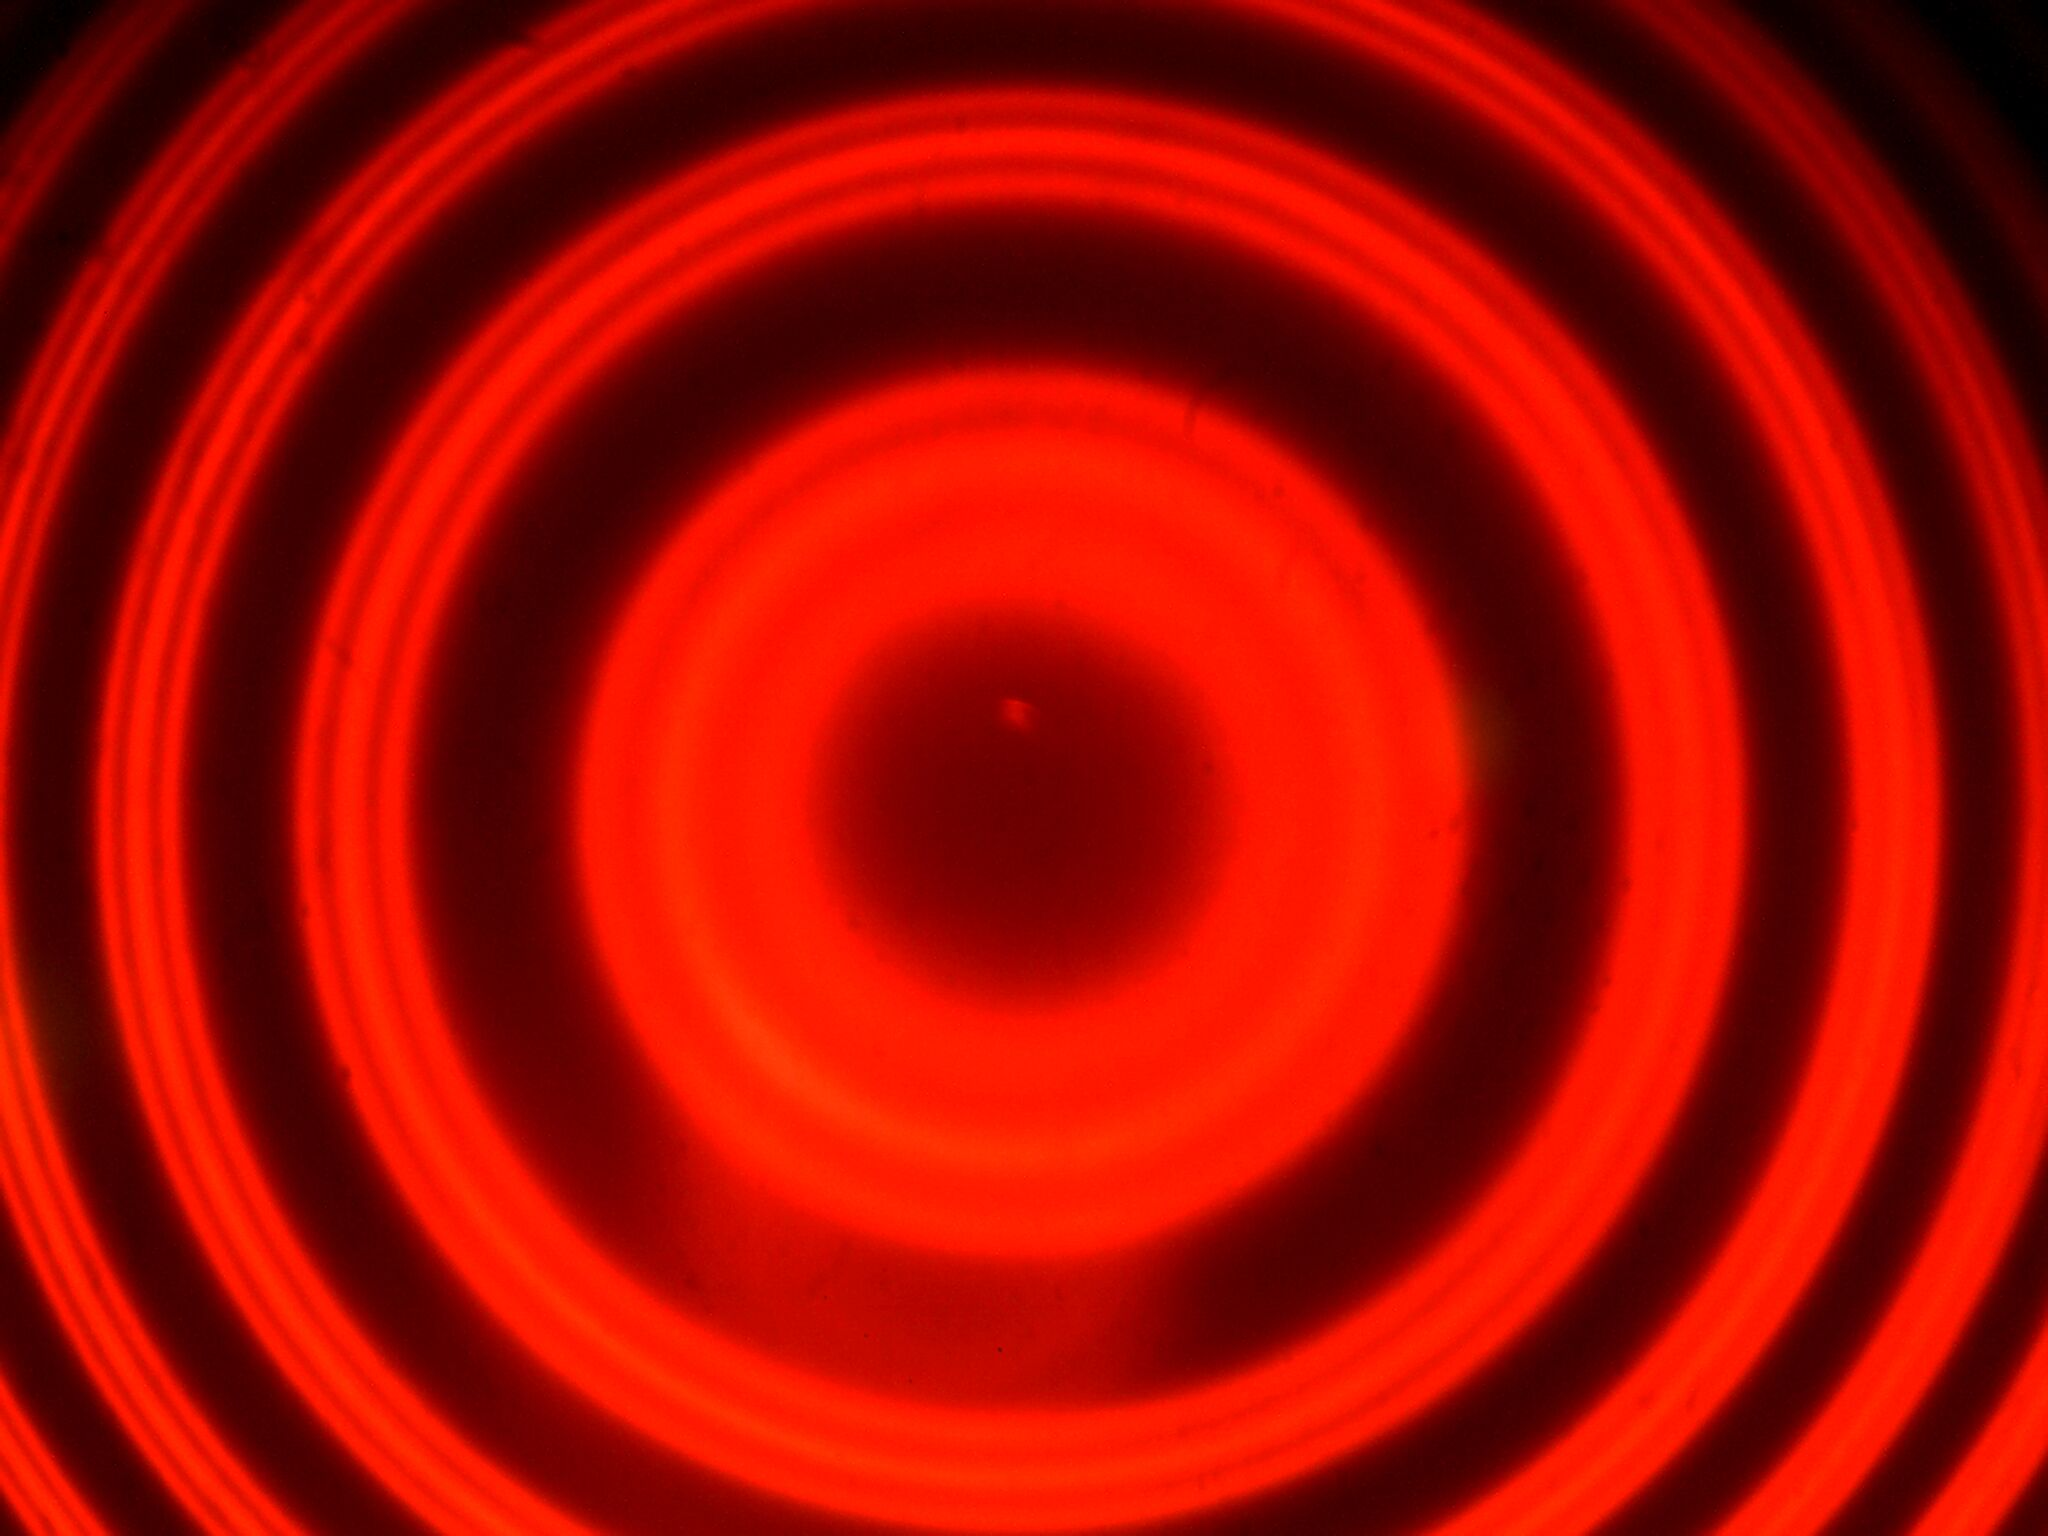
\includegraphics[width=0.45\textwidth]{images/Capture_816.bmp.jpg}
	    \hspace{1em}
	    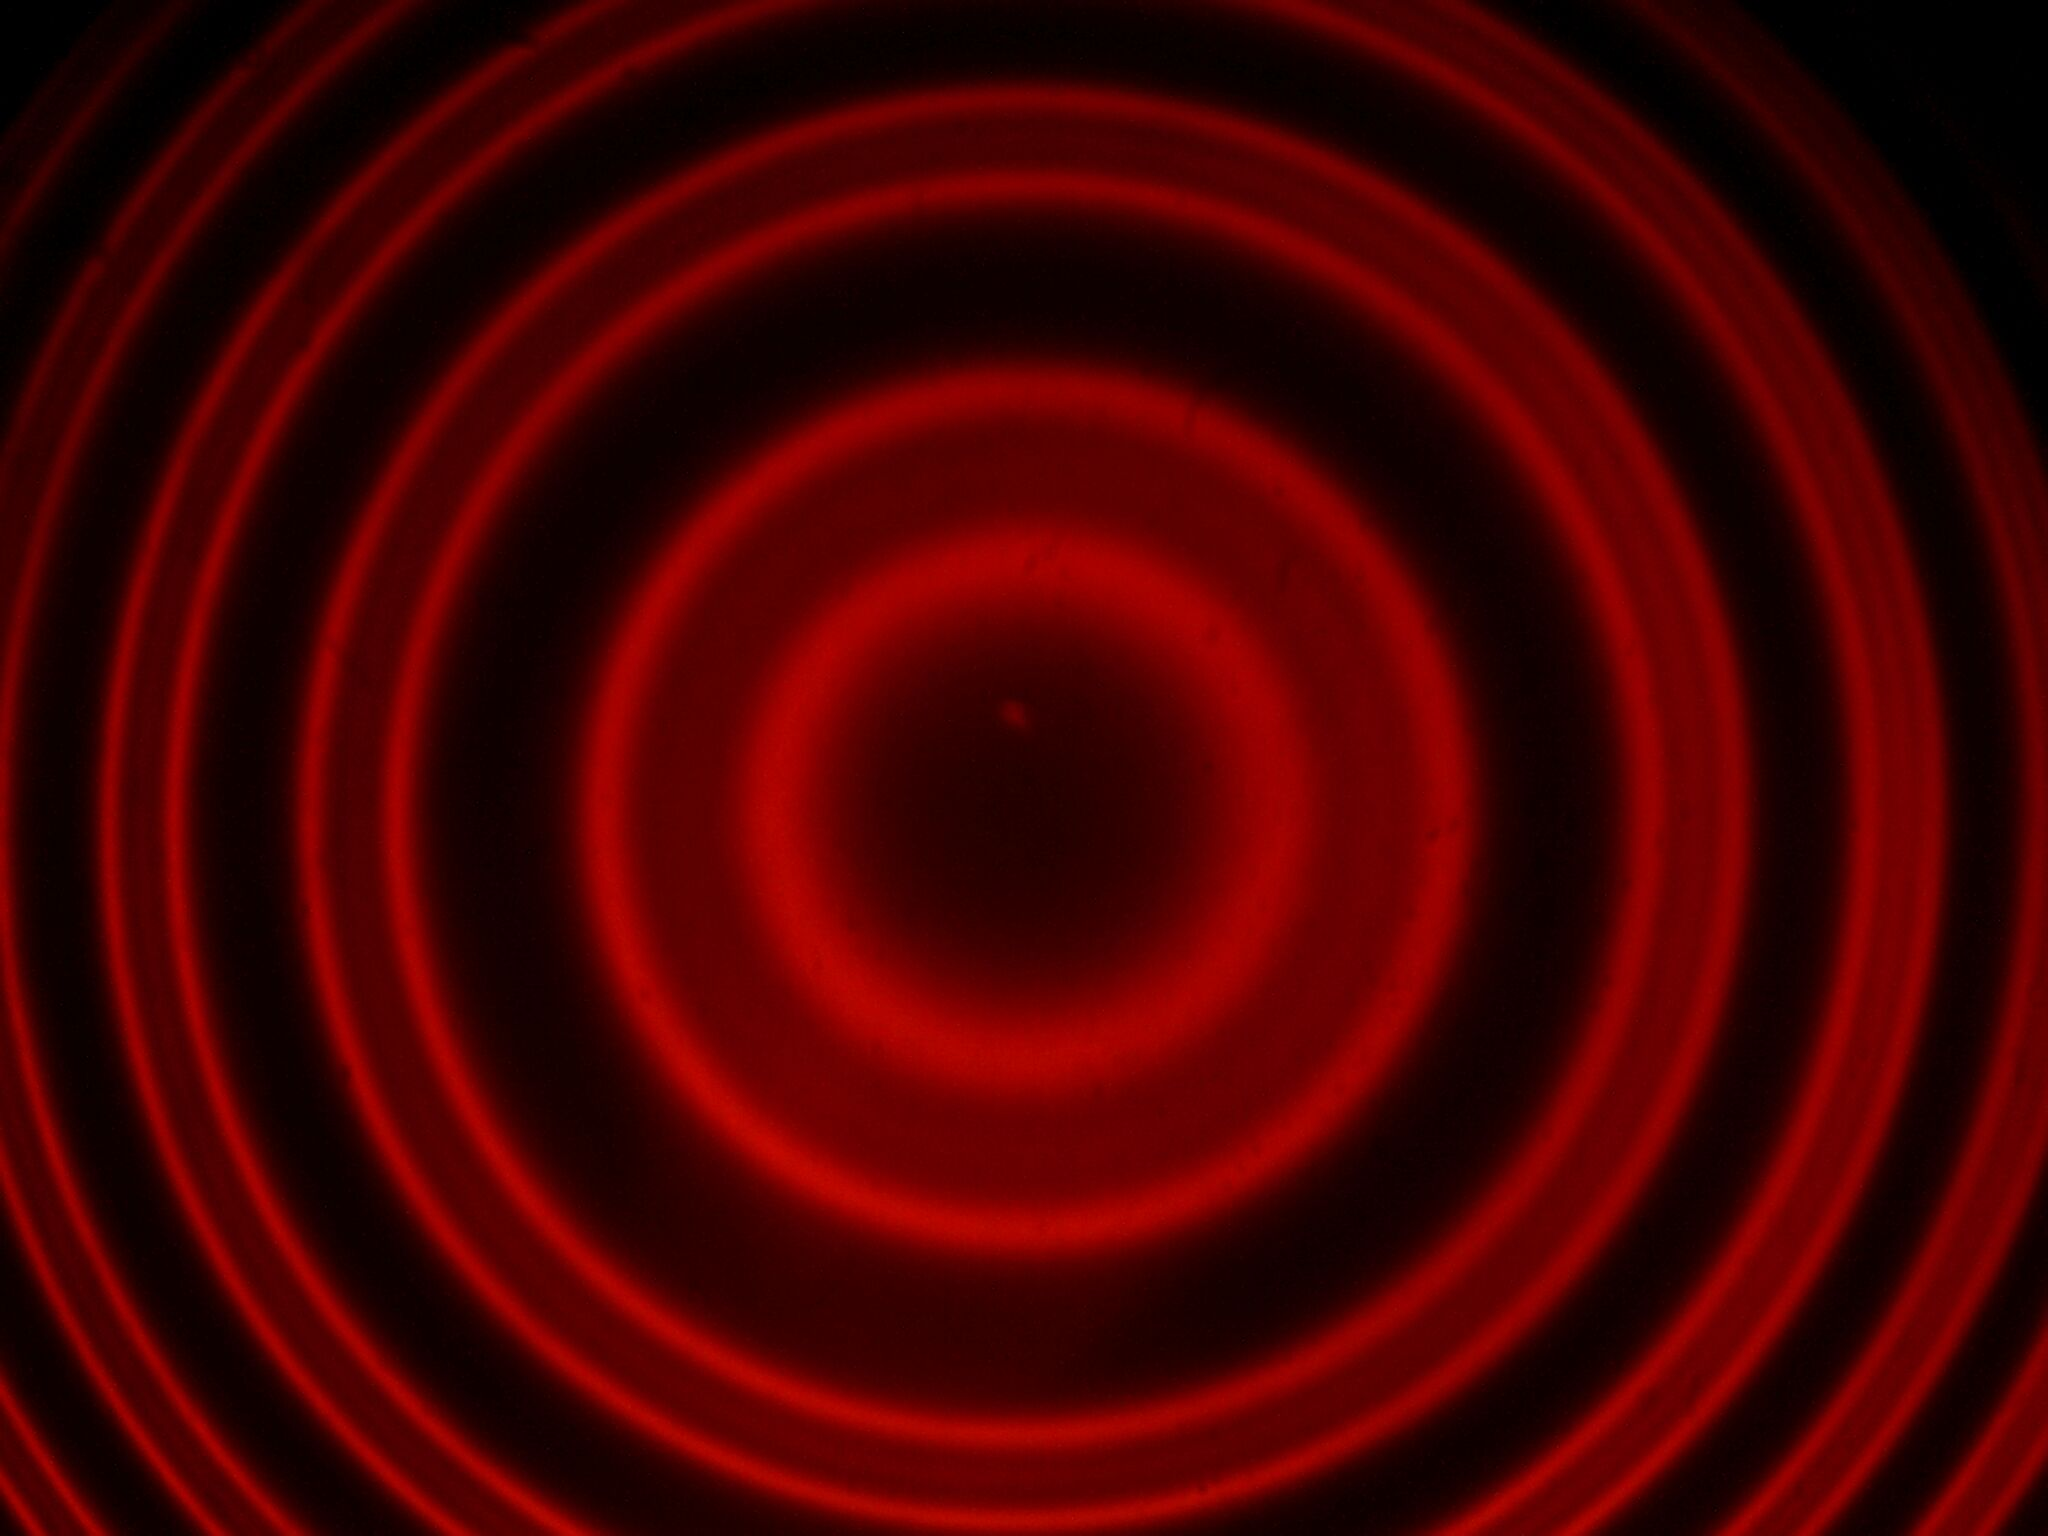
\includegraphics[width=0.45\textwidth]{images/Capture_815.bmp.jpg}
	    \caption{Interferenzringe von rote Emissionslinie im Magnetfeld $B \approx  \SI{6}{\ampere}$. Ohne Polarisationsfilter (Links). Mit Polarisationsfilter (Rechts)}
	    \label{fig:red-fringes-pol-B-big}
	    \vspace{-0.5em}
	\end{figure}
	\newpage
	\begin{figure}[!ht]
	    \centering
	   	\begin{subfigure}{0.48\textwidth}
			\centering
			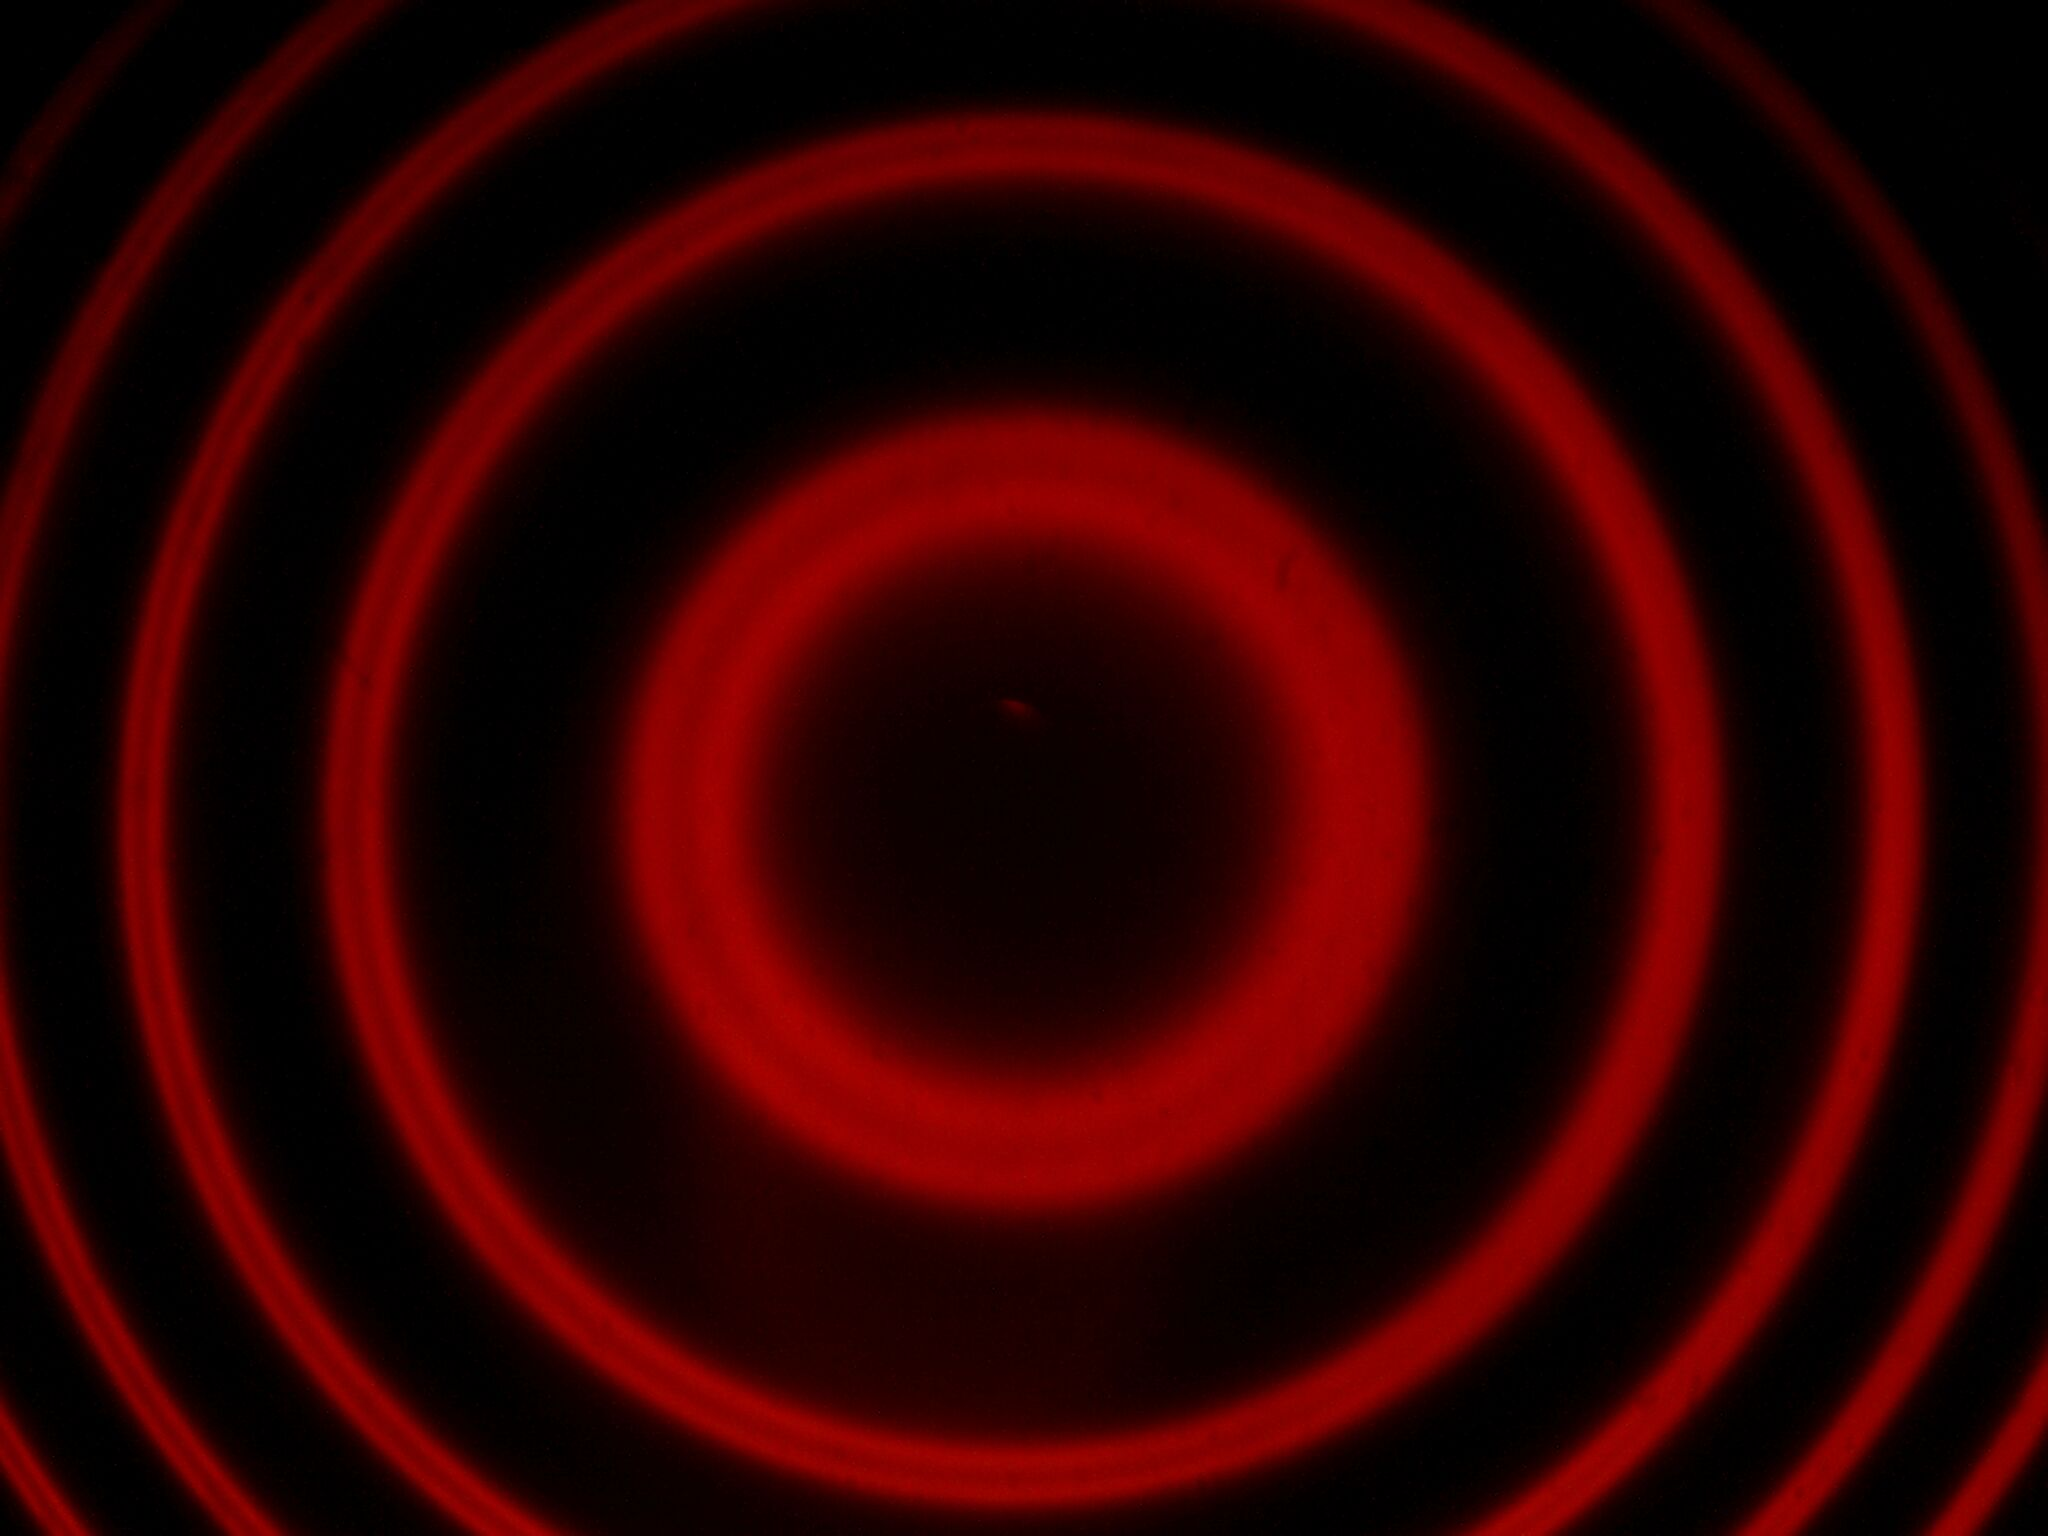
\includegraphics[width=\textwidth]{images/Capture_817.bmp.jpg}
			\caption{$I = \SI{2.495(5)}{\ampere}$}
			\label{fig:red_I2.495}
			\vspace{0.5\baselineskip}
		\end{subfigure}
		\hfill
		\begin{subfigure}{0.48\textwidth}
			\centering
			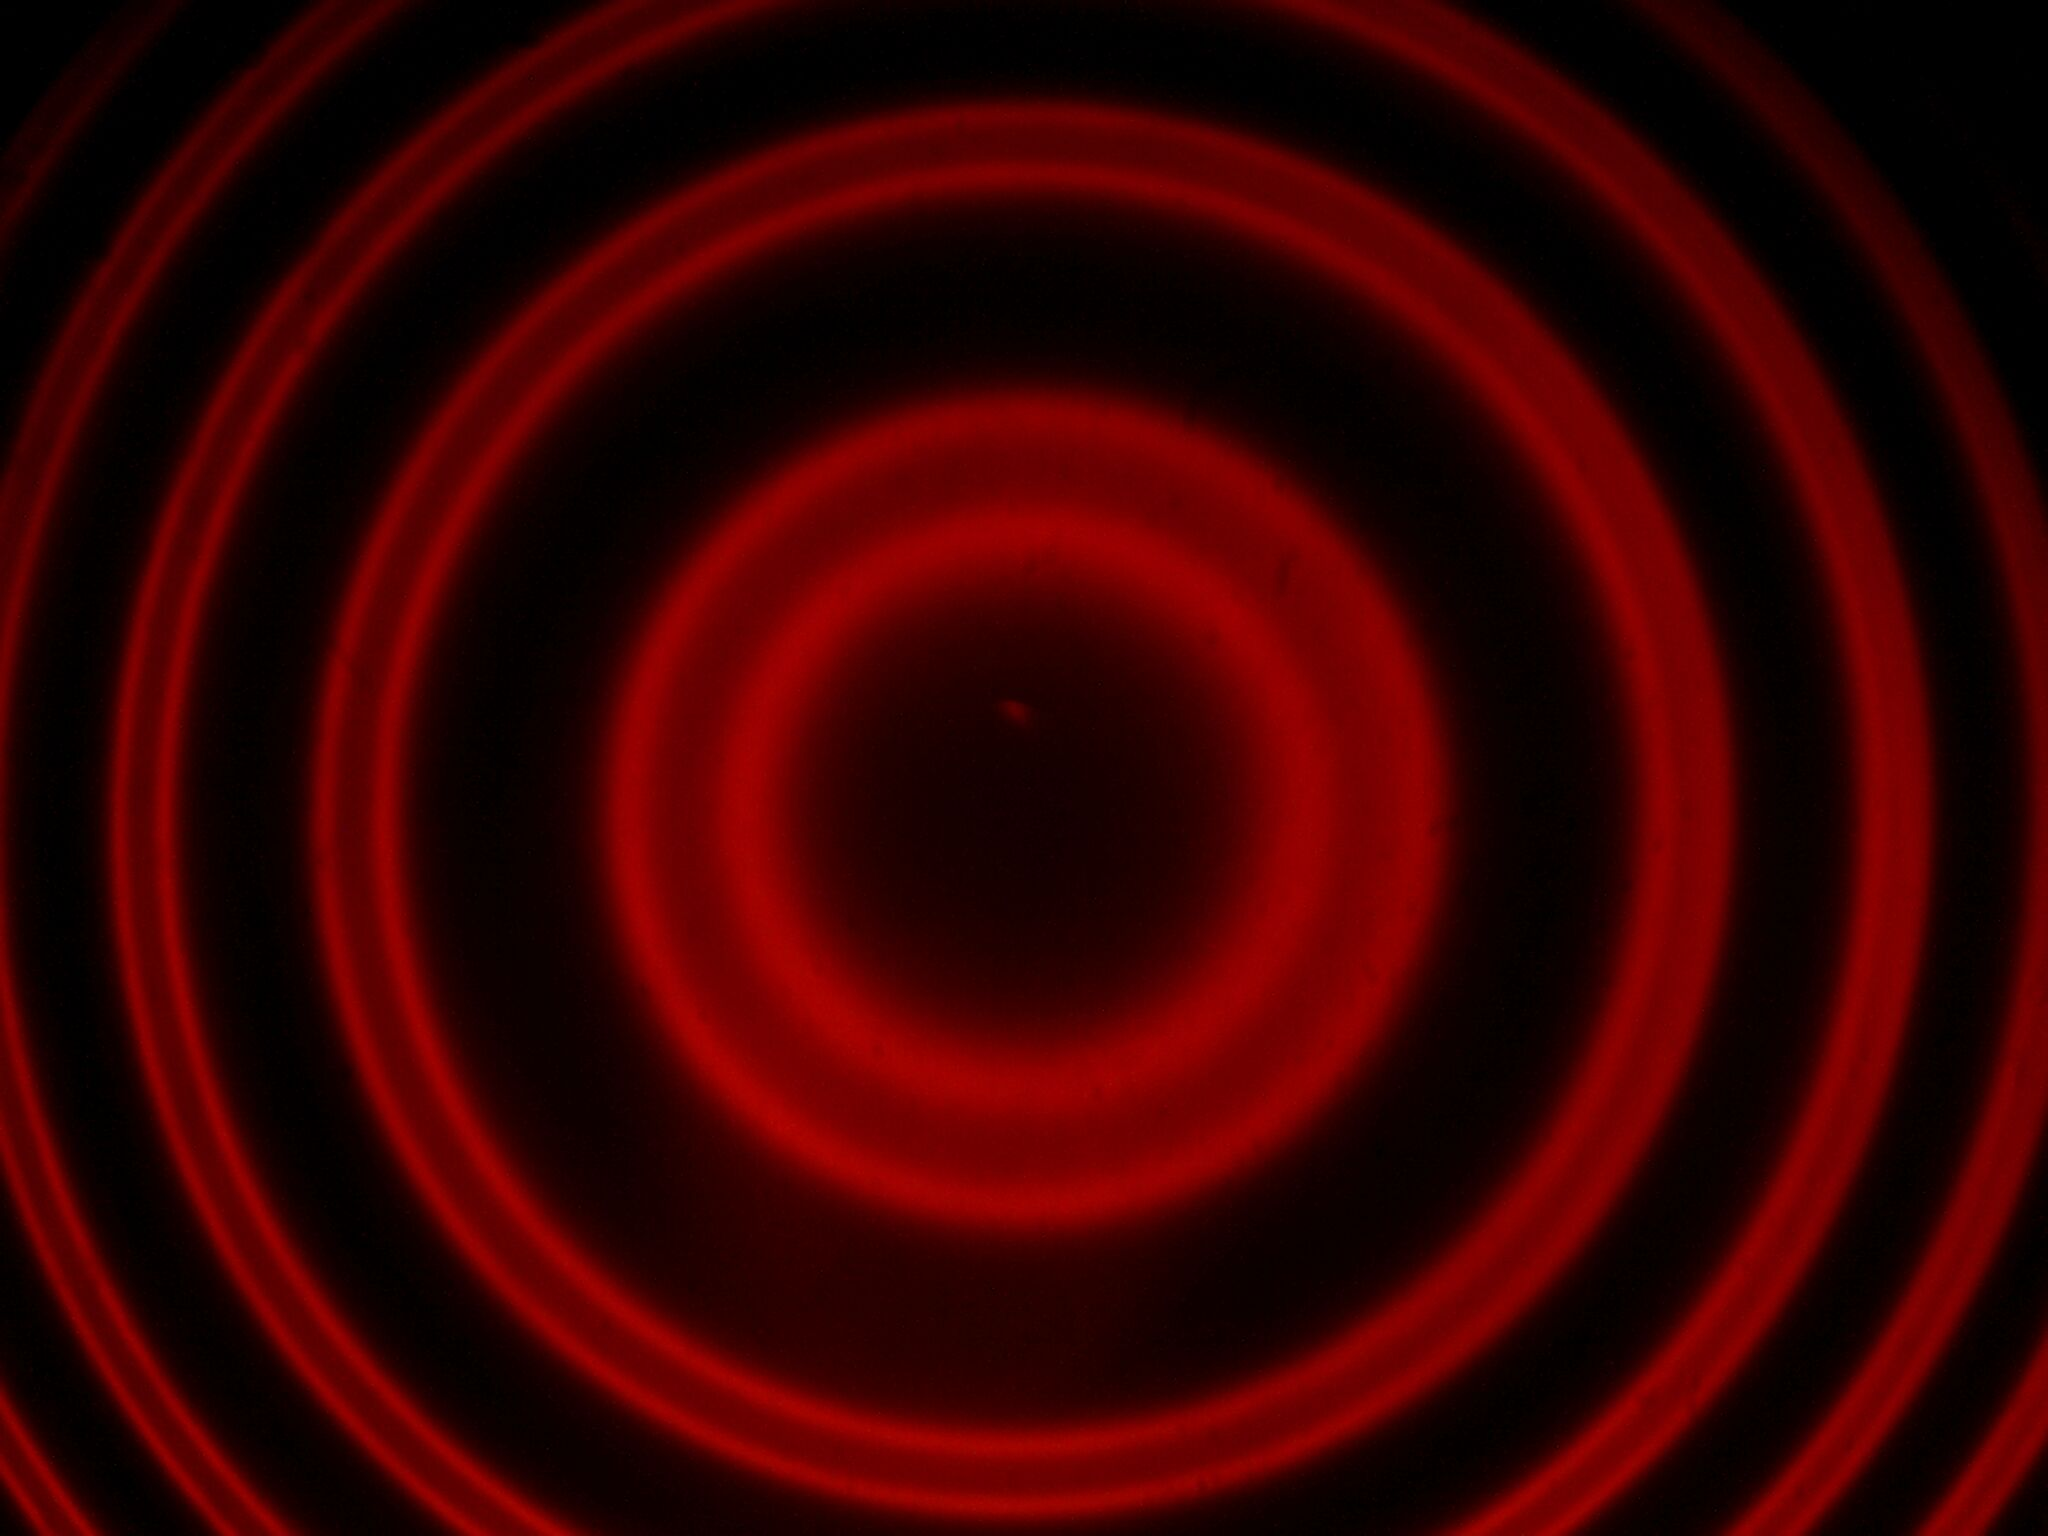
\includegraphics[width=\textwidth]{images/Capture_818.bmp.jpg}
			\caption{$I = \SI{4.190(10)}{\ampere}$}
			\label{fig:red_I4190}
			\vspace{0.5\baselineskip}
		\end{subfigure}
		\begin{subfigure}{0.48\textwidth}
			\centering
			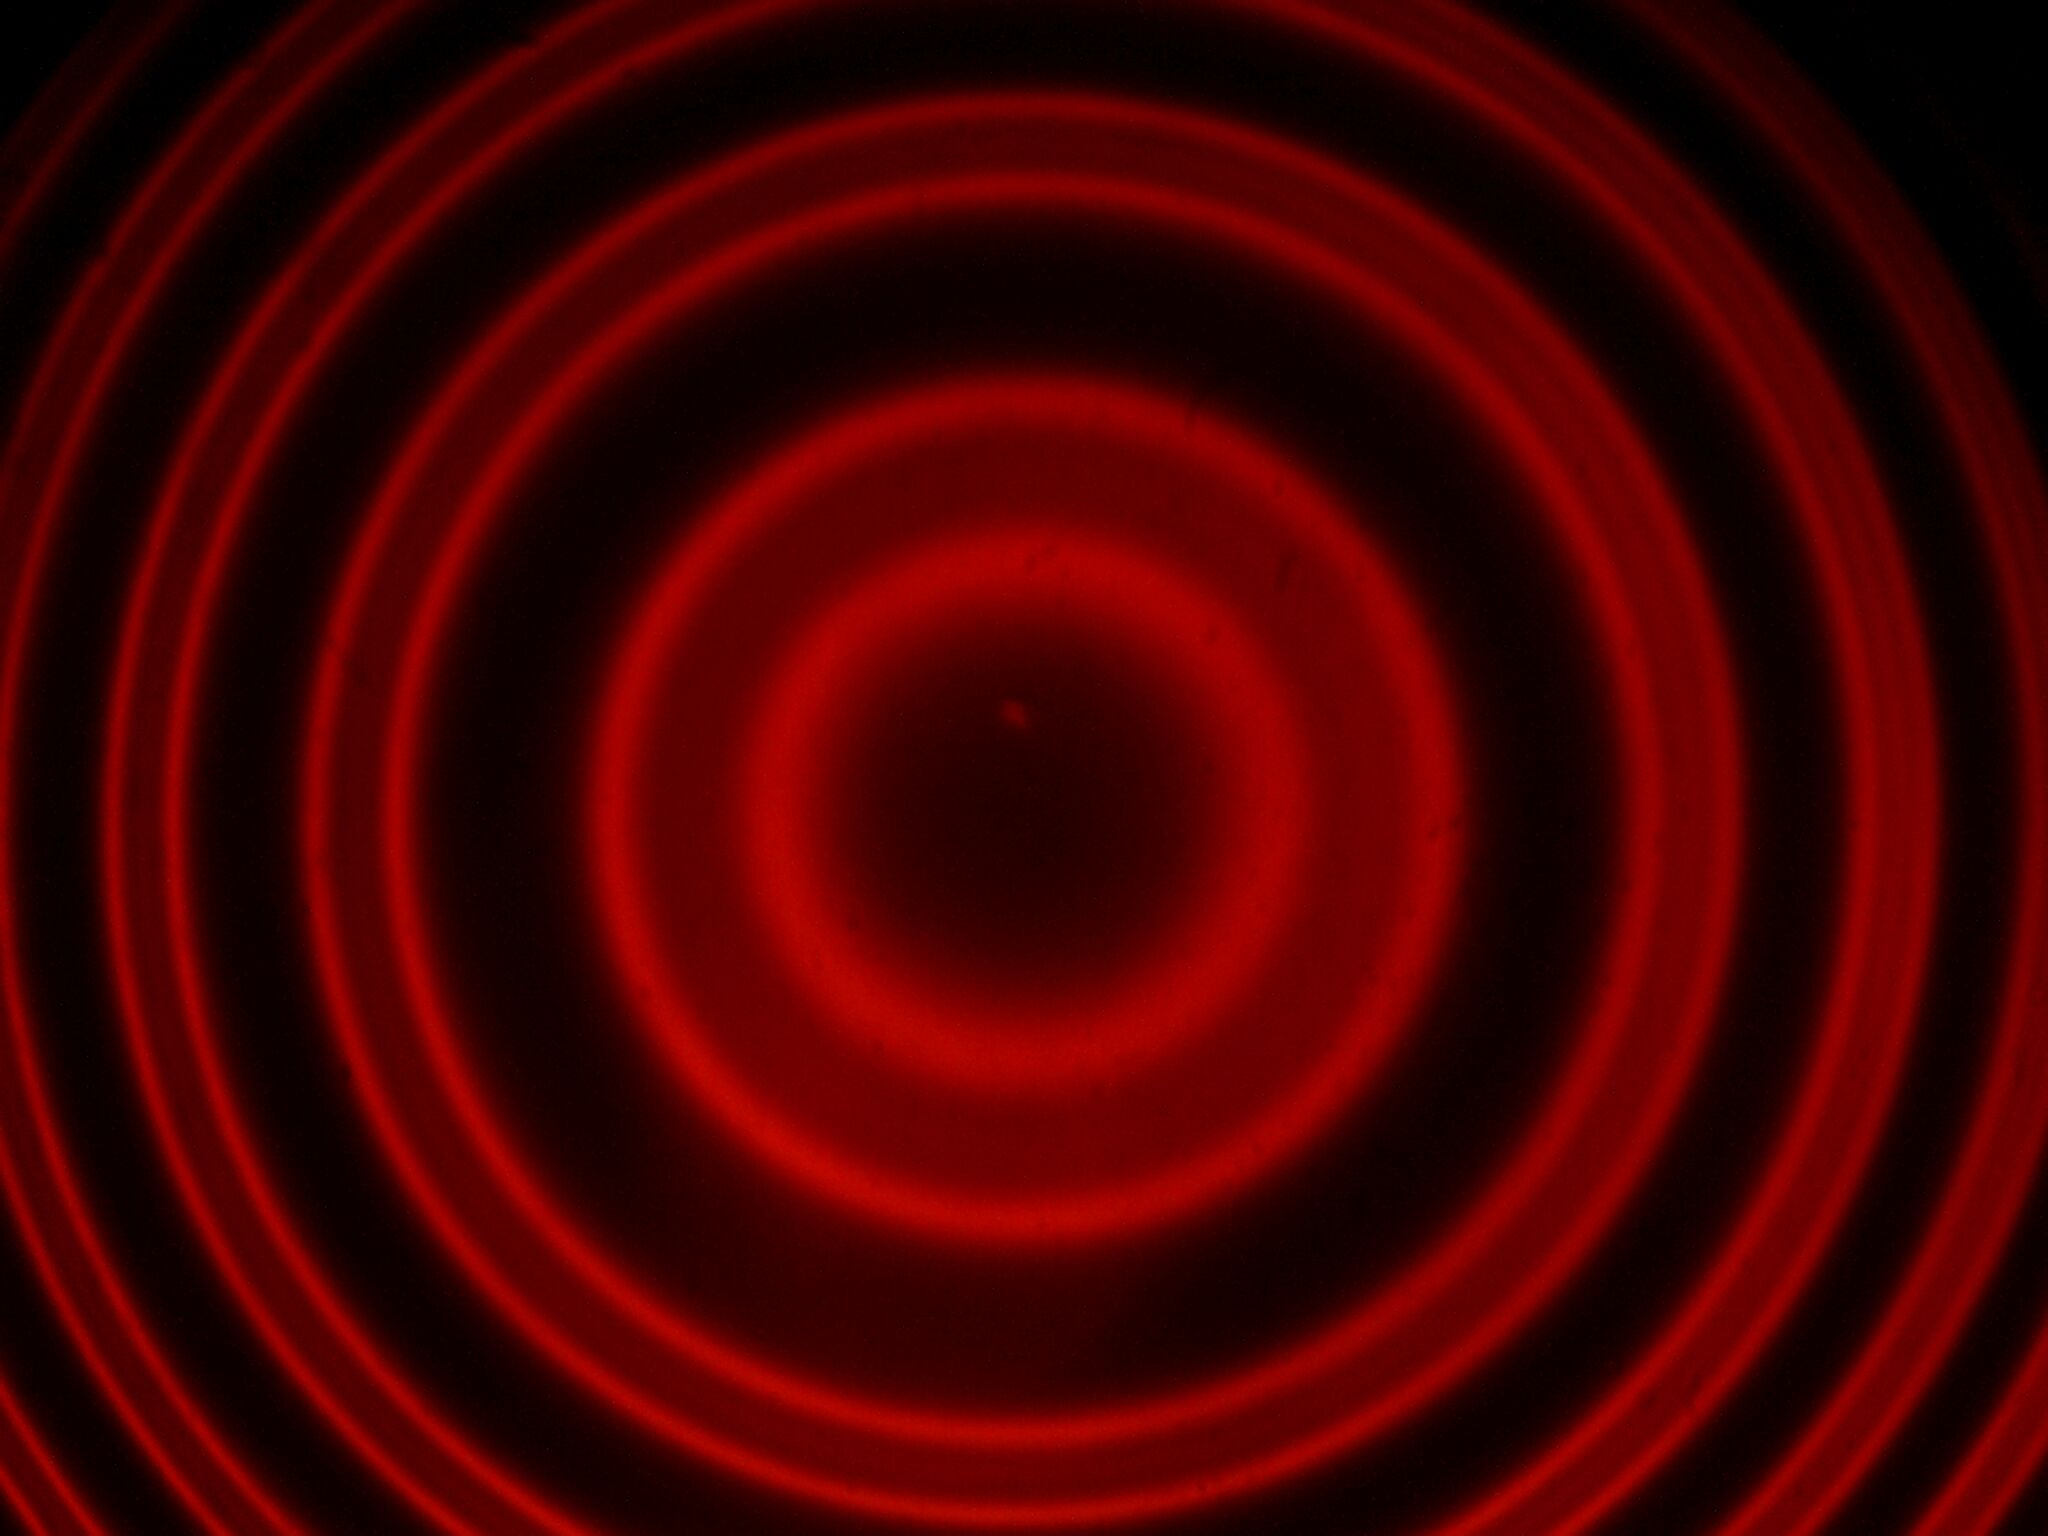
\includegraphics[width=\textwidth]{images/Capture_819.bmp.jpg}
			\caption{$I = \SI{5.662(10)}{\ampere}$}
			\label{fig:red_I5.662}
			\vspace{0.5\baselineskip}
		\end{subfigure}
		\hfill
		\begin{subfigure}{0.48\textwidth}
			\centering
			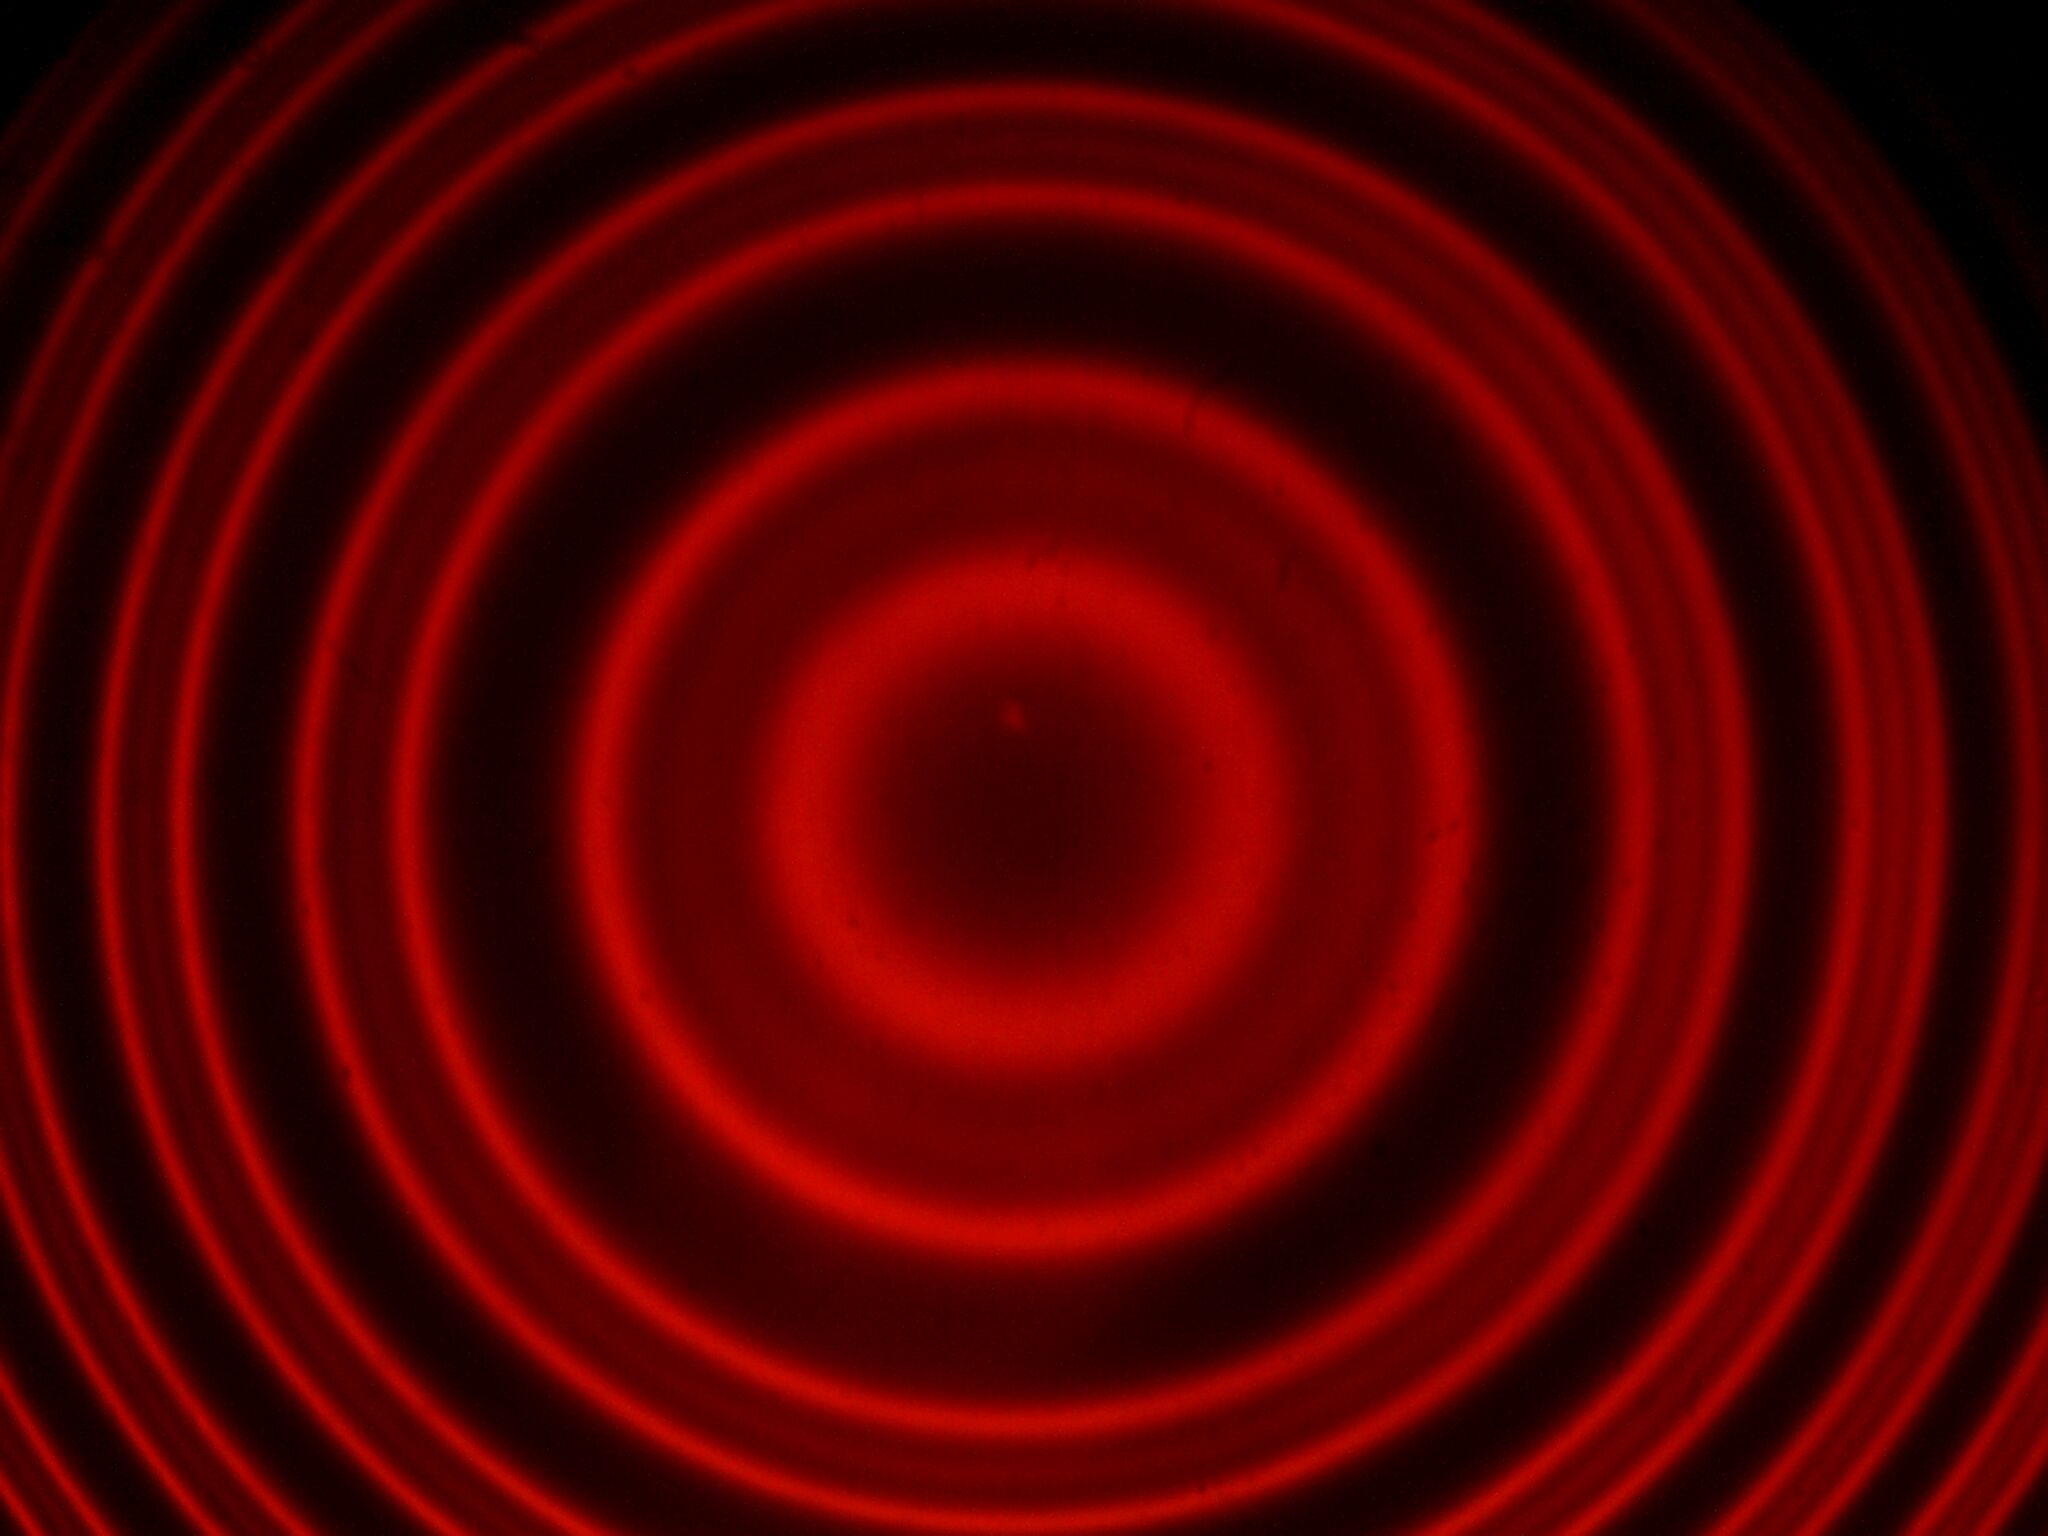
\includegraphics[width=\textwidth]{images/Capture_820.bmp.jpg}
			\caption{$I = \SI{7.01(1)}{\ampere}$}
			\label{fig:red_I7.01}
			\vspace{0.5\baselineskip}
		\end{subfigure}
		\begin{subfigure}{0.48\textwidth}
			\centering
			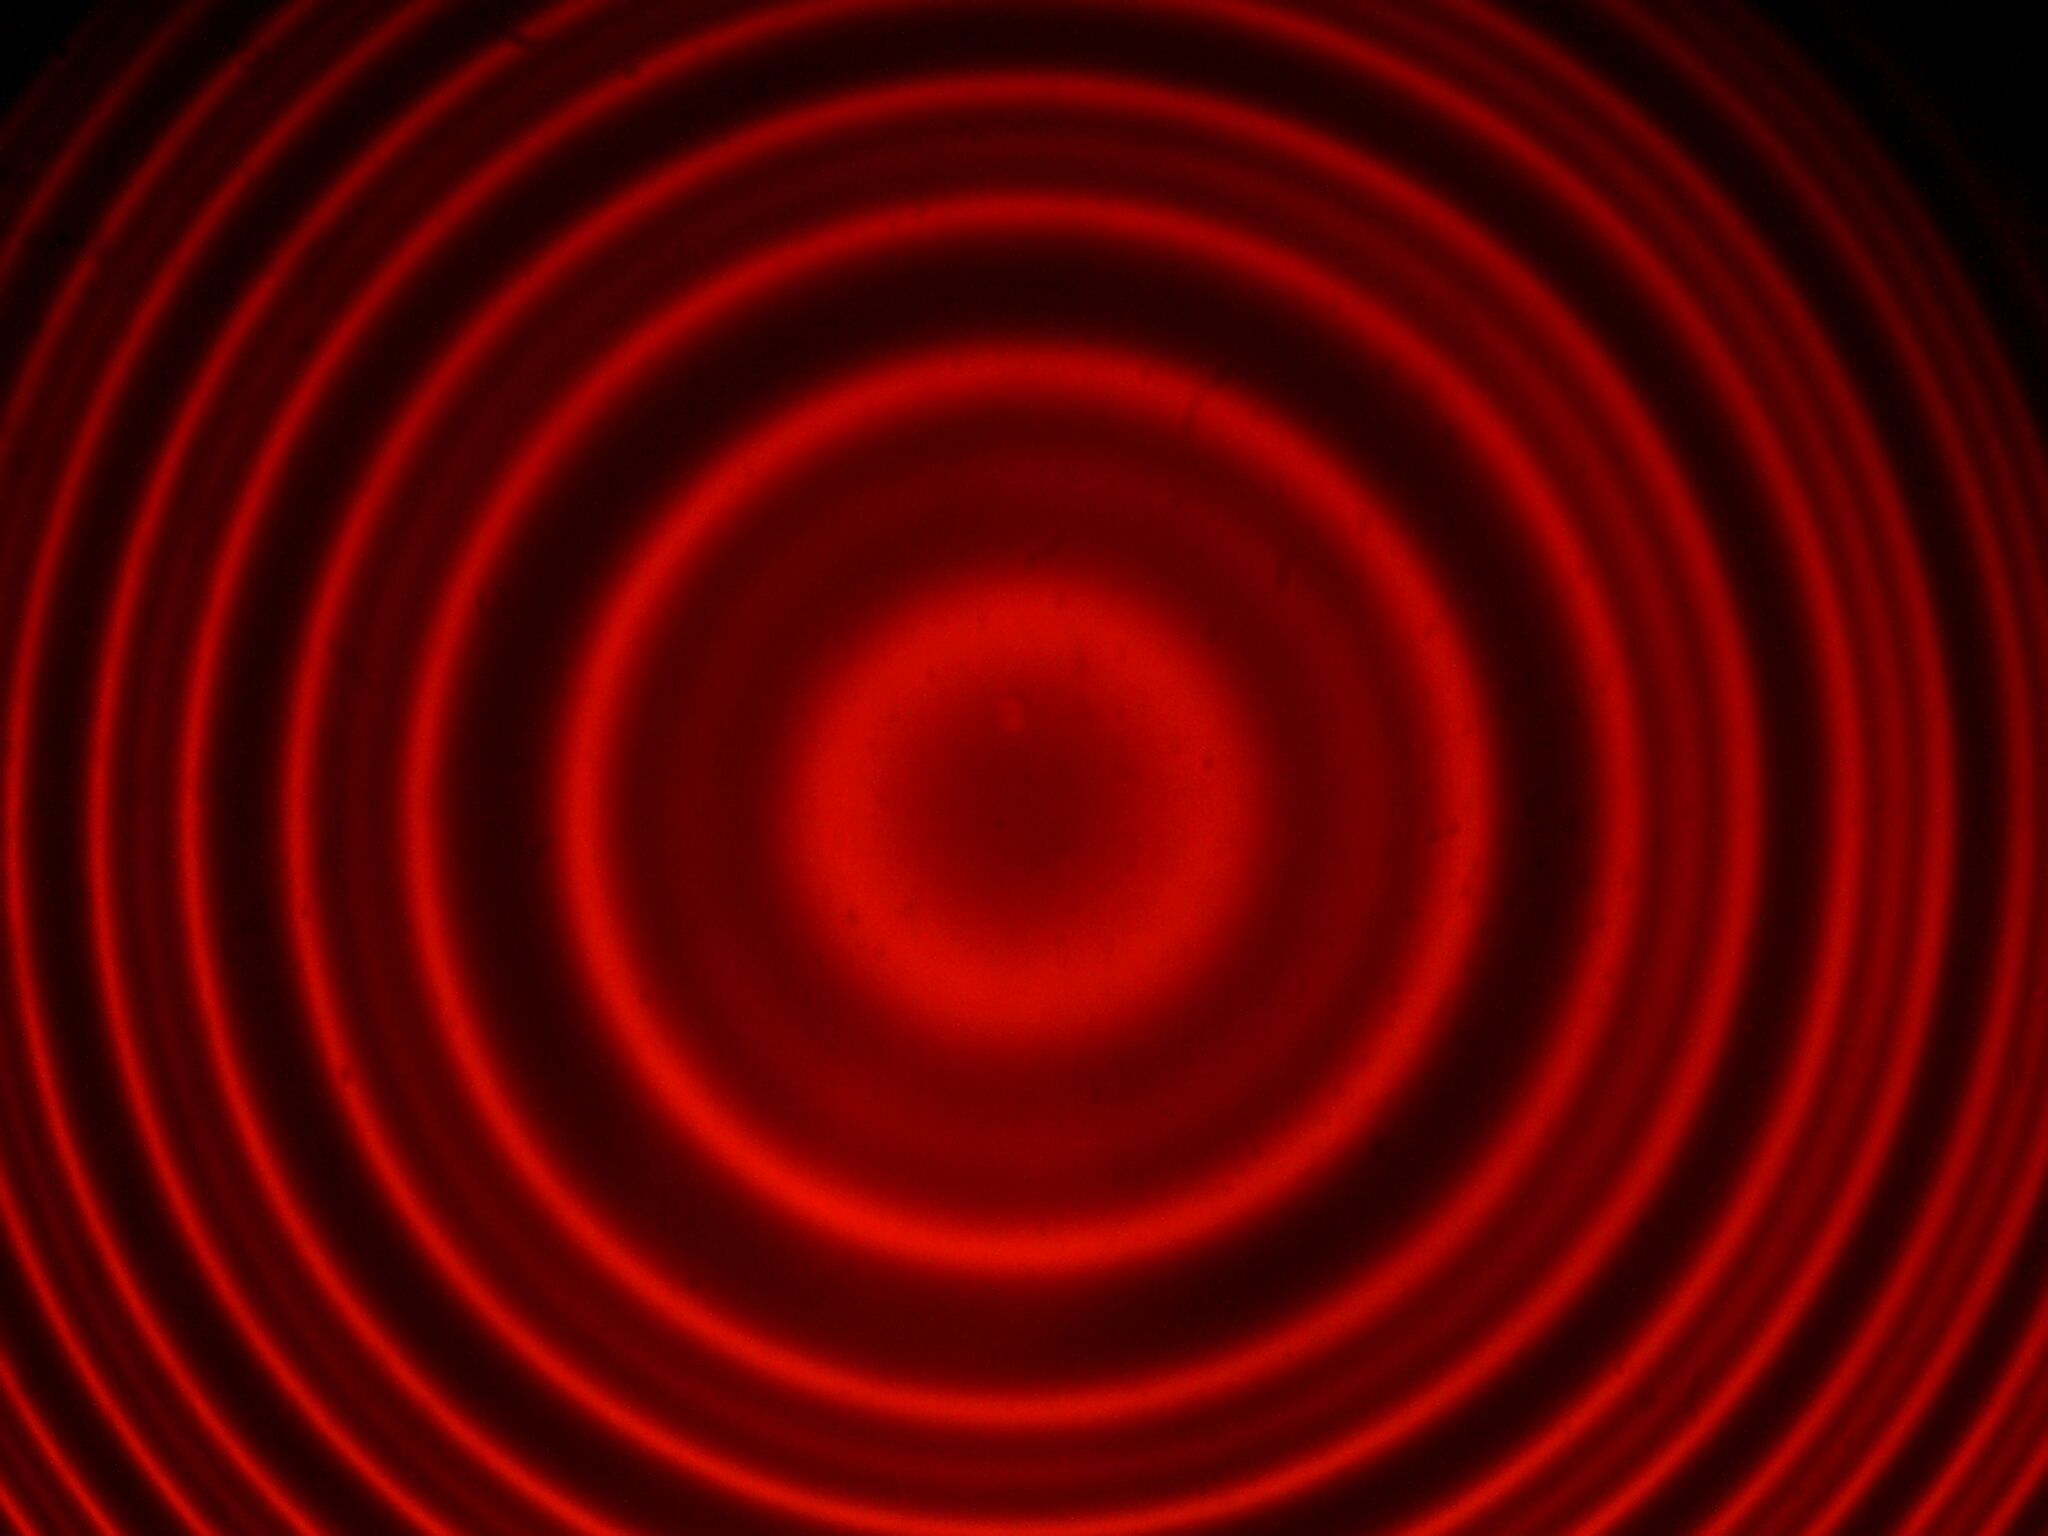
\includegraphics[width=\textwidth]{images/Capture_821.bmp.jpg}
			\caption{$I = \SI{8.78(1)}{\ampere}$}
			\label{fig:red_I8.78}
		\end{subfigure}
	    \caption{Messungen}
	    \label{fig:tv4-messungen}
	\end{figure}
	\newpage
	Da die Messreihe zu lang ist, wird sie hier nicht wieder formatiert. Sie finden die Messreihe im Laborprotokoll unter Teilversuch 4. Alle Rechnungen für $r_m^2$ und $\Delta r_m^2 = 2r_m(\Delta r_m)$ werden direkt in \gnuplot{} berechnet und somit hier nicht weiter beschrieben. 

	Wir führe nun die benötigte Kurveanpassungen zu $r_m^2 = mp + c$ durch. Der $p$-Achsenschnittpunkt $p_0$ ist somit gegeben durch:
	\begin{align}
		p_0 &= -\frac{c}{m} \\
		\Delta p_0 &= |p_0|\relquad{c,m}
	\end{align}
	und im \gnuplot{} direkt berechnet. 

	Für $\lambda_-$:
	\begin{figure}[!ht]
	    \centering
	    \vspace{-0.5em}
	    % https://tex.stackexchange.com/a/98142
	    \resizebox{6in}{!}{% GNUPLOT: LaTeX picture with Postscript
\begingroup
  \makeatletter
  \providecommand\color[2][]{%
    \GenericError{(gnuplot) \space\space\space\@spaces}{%
      Package color not loaded in conjunction with
      terminal option `colourtext'%
    }{See the gnuplot documentation for explanation.%
    }{Either use 'blacktext' in gnuplot or load the package
      color.sty in LaTeX.}%
    \renewcommand\color[2][]{}%
  }%
  \providecommand\includegraphics[2][]{%
    \GenericError{(gnuplot) \space\space\space\@spaces}{%
      Package graphicx or graphics not loaded%
    }{See the gnuplot documentation for explanation.%
    }{The gnuplot epslatex terminal needs graphicx.sty or graphics.sty.}%
    \renewcommand\includegraphics[2][]{}%
  }%
  \providecommand\rotatebox[2]{#2}%
  \@ifundefined{ifGPcolor}{%
    \newif\ifGPcolor
    \GPcolortrue
  }{}%
  \@ifundefined{ifGPblacktext}{%
    \newif\ifGPblacktext
    \GPblacktexttrue
  }{}%
  % define a \g@addto@macro without @ in the name:
  \let\gplgaddtomacro\g@addto@macro
  % define empty templates for all commands taking text:
  \gdef\gplbacktext{}%
  \gdef\gplfronttext{}%
  \makeatother
  \ifGPblacktext
    % no textcolor at all
    \def\colorrgb#1{}%
    \def\colorgray#1{}%
  \else
    % gray or color?
    \ifGPcolor
      \def\colorrgb#1{\color[rgb]{#1}}%
      \def\colorgray#1{\color[gray]{#1}}%
      \expandafter\def\csname LTw\endcsname{\color{white}}%
      \expandafter\def\csname LTb\endcsname{\color{black}}%
      \expandafter\def\csname LTa\endcsname{\color{black}}%
      \expandafter\def\csname LT0\endcsname{\color[rgb]{1,0,0}}%
      \expandafter\def\csname LT1\endcsname{\color[rgb]{0,1,0}}%
      \expandafter\def\csname LT2\endcsname{\color[rgb]{0,0,1}}%
      \expandafter\def\csname LT3\endcsname{\color[rgb]{1,0,1}}%
      \expandafter\def\csname LT4\endcsname{\color[rgb]{0,1,1}}%
      \expandafter\def\csname LT5\endcsname{\color[rgb]{1,1,0}}%
      \expandafter\def\csname LT6\endcsname{\color[rgb]{0,0,0}}%
      \expandafter\def\csname LT7\endcsname{\color[rgb]{1,0.3,0}}%
      \expandafter\def\csname LT8\endcsname{\color[rgb]{0.5,0.5,0.5}}%
    \else
      % gray
      \def\colorrgb#1{\color{black}}%
      \def\colorgray#1{\color[gray]{#1}}%
      \expandafter\def\csname LTw\endcsname{\color{white}}%
      \expandafter\def\csname LTb\endcsname{\color{black}}%
      \expandafter\def\csname LTa\endcsname{\color{black}}%
      \expandafter\def\csname LT0\endcsname{\color{black}}%
      \expandafter\def\csname LT1\endcsname{\color{black}}%
      \expandafter\def\csname LT2\endcsname{\color{black}}%
      \expandafter\def\csname LT3\endcsname{\color{black}}%
      \expandafter\def\csname LT4\endcsname{\color{black}}%
      \expandafter\def\csname LT5\endcsname{\color{black}}%
      \expandafter\def\csname LT6\endcsname{\color{black}}%
      \expandafter\def\csname LT7\endcsname{\color{black}}%
      \expandafter\def\csname LT8\endcsname{\color{black}}%
    \fi
  \fi
    \setlength{\unitlength}{0.0500bp}%
    \ifx\gptboxheight\undefined%
      \newlength{\gptboxheight}%
      \newlength{\gptboxwidth}%
      \newsavebox{\gptboxtext}%
    \fi%
    \setlength{\fboxrule}{0.5pt}%
    \setlength{\fboxsep}{1pt}%
    \definecolor{tbcol}{rgb}{1,1,1}%
\begin{picture}(10080.00,6480.00)%
    \gplgaddtomacro\gplbacktext{%
      \csname LTb\endcsname%%
      \put(1078,704){\makebox(0,0)[r]{\strut{}$0$}}%
      \put(1078,1435){\makebox(0,0)[r]{\strut{}$5000$}}%
      \put(1078,2165){\makebox(0,0)[r]{\strut{}$10000$}}%
      \put(1078,2896){\makebox(0,0)[r]{\strut{}$15000$}}%
      \put(1078,3627){\makebox(0,0)[r]{\strut{}$20000$}}%
      \put(1078,4358){\makebox(0,0)[r]{\strut{}$25000$}}%
      \put(1078,5088){\makebox(0,0)[r]{\strut{}$30000$}}%
      \put(1078,5819){\makebox(0,0)[r]{\strut{}$35000$}}%
      \put(1210,484){\makebox(0,0){\strut{}$1$}}%
      \put(2269,484){\makebox(0,0){\strut{}$1,5$}}%
      \put(3328,484){\makebox(0,0){\strut{}$2$}}%
      \put(4387,484){\makebox(0,0){\strut{}$2,5$}}%
      \put(5447,484){\makebox(0,0){\strut{}$3$}}%
      \put(6506,484){\makebox(0,0){\strut{}$3,5$}}%
      \put(7565,484){\makebox(0,0){\strut{}$4$}}%
      \put(8624,484){\makebox(0,0){\strut{}$4,5$}}%
      \put(9683,484){\makebox(0,0){\strut{}$5$}}%
    }%
    \gplgaddtomacro\gplfronttext{%
      \csname LTb\endcsname%%
      \put(209,3261){\rotatebox{-270}{\makebox(0,0){\strut{}Radien$^2$ $r_m^2/\si{\micro\meter\squared}$}}}%
      \put(5446,154){\makebox(0,0){\strut{}Ringindex $p$ (Einheitlos)}}%
      \csname LTb\endcsname%%
      \put(5201,1757){\makebox(0,0)[r]{\strut{}$I = \SI{2.495(5)}{\ampere}$}}%
      \csname LTb\endcsname%%
      \put(5201,1537){\makebox(0,0)[r]{\strut{}$I = \SI{4.190(10)}{\ampere}$}}%
      \csname LTb\endcsname%%
      \put(5201,1317){\makebox(0,0)[r]{\strut{}$I = \SI{5.662(10)}{\ampere}$}}%
      \csname LTb\endcsname%%
      \put(5201,1097){\makebox(0,0)[r]{\strut{}$I = \SI{7.01(1)}{\ampere}$}}%
      \csname LTb\endcsname%%
      \put(5201,877){\makebox(0,0)[r]{\strut{}$I = \SI{8.78(1)}{\ampere}$}}%
      \csname LTb\endcsname%%
      \put(8696,1757){\makebox(0,0)[r]{\strut{}$7819,48208p + (-5456,66280)$}}%
      \csname LTb\endcsname%%
      \put(8696,1537){\makebox(0,0)[r]{\strut{}$7842,83447p + (-5913,98932)$}}%
      \csname LTb\endcsname%%
      \put(8696,1317){\makebox(0,0)[r]{\strut{}$7817,57179p + (-6241,75284)$}}%
      \csname LTb\endcsname%%
      \put(8696,1097){\makebox(0,0)[r]{\strut{}$7793,98133p + (-6489,22780)$}}%
      \csname LTb\endcsname%%
      \put(8696,877){\makebox(0,0)[r]{\strut{}$7788,40259p + (-6803,03677)$}}%
      \csname LTb\endcsname%%
      \put(5446,6149){\makebox(0,0){\strut{}Verlauf der Radien mit Ringenindizes ($\lambda_-$)}}%
    }%
    \gplbacktext
    \put(0,0){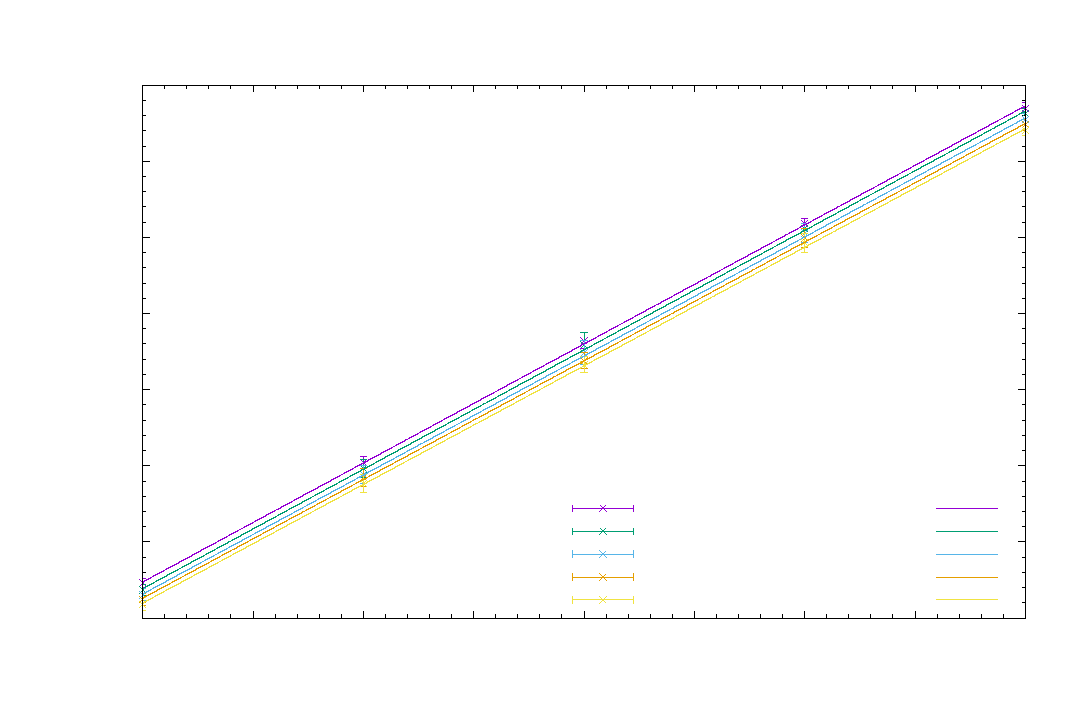
\includegraphics[width={504.00bp},height={324.00bp}]{tv4-l-minus}}%
    \gplfronttext
  \end{picture}%
\endgroup
}
	    \caption{Verlauf der Ringradien}
	    \label{fig:tv4-l-minus}
	    \vspace{-0.5em}
	\end{figure}
	\begin{center}
		\begin{tabular}{lrrrr}
			\toprule
			Strom $I/\si{\ampere}$ & $m/\si{\micro\meter\squared}$ & $c/\si{\micro\meter\squared}$ & $p_0$ & $\chi^2_\text{red}$ \\
			\midrule
	        \num{2.495(5)} & \num{7819,48208(4158214)} & \num{-5456,66280(13503726)} & \num{0,69783(1766)} & \num{0,16085} \\
	        \num{4.190(10)} & \num{7842,83447(5429714)} & \num{-5913,98932(19243657)} & \num{0,75406(2509)} & \num{0,22324} \\
	        \num{5.662(10)} & \num{7817,57179(4049964)} & \num{-6241,75284(14258167)} & \num{0,79843(1870)} & \num{0,10189} \\
	        \num{7.01(1)} & \num{7793,98133(4273437)} & \num{-6489,22780(15147792)} & \num{0,83259(1996)} & \num{0,10681} \\
	        \num{8.78(1)} & \num{7788,40259(4619194)} & \num{-6803,03677(16369671)} & \num{0,87348(2165)} & \num{0,12585} \\
			\bottomrule
		\end{tabular}
	\end{center}
	Die kleine $\chi^2_\text{red}$'s zeigt eine gute Kurveanpassung. 

	Für $\lambda_+$:
	\begin{figure}[!ht]
	    \centering
	    \vspace{-0.5em}
	    % https://tex.stackexchange.com/a/98142
	    \resizebox{6in}{!}{% GNUPLOT: LaTeX picture with Postscript
\begingroup
  \makeatletter
  \providecommand\color[2][]{%
    \GenericError{(gnuplot) \space\space\space\@spaces}{%
      Package color not loaded in conjunction with
      terminal option `colourtext'%
    }{See the gnuplot documentation for explanation.%
    }{Either use 'blacktext' in gnuplot or load the package
      color.sty in LaTeX.}%
    \renewcommand\color[2][]{}%
  }%
  \providecommand\includegraphics[2][]{%
    \GenericError{(gnuplot) \space\space\space\@spaces}{%
      Package graphicx or graphics not loaded%
    }{See the gnuplot documentation for explanation.%
    }{The gnuplot epslatex terminal needs graphicx.sty or graphics.sty.}%
    \renewcommand\includegraphics[2][]{}%
  }%
  \providecommand\rotatebox[2]{#2}%
  \@ifundefined{ifGPcolor}{%
    \newif\ifGPcolor
    \GPcolortrue
  }{}%
  \@ifundefined{ifGPblacktext}{%
    \newif\ifGPblacktext
    \GPblacktexttrue
  }{}%
  % define a \g@addto@macro without @ in the name:
  \let\gplgaddtomacro\g@addto@macro
  % define empty templates for all commands taking text:
  \gdef\gplbacktext{}%
  \gdef\gplfronttext{}%
  \makeatother
  \ifGPblacktext
    % no textcolor at all
    \def\colorrgb#1{}%
    \def\colorgray#1{}%
  \else
    % gray or color?
    \ifGPcolor
      \def\colorrgb#1{\color[rgb]{#1}}%
      \def\colorgray#1{\color[gray]{#1}}%
      \expandafter\def\csname LTw\endcsname{\color{white}}%
      \expandafter\def\csname LTb\endcsname{\color{black}}%
      \expandafter\def\csname LTa\endcsname{\color{black}}%
      \expandafter\def\csname LT0\endcsname{\color[rgb]{1,0,0}}%
      \expandafter\def\csname LT1\endcsname{\color[rgb]{0,1,0}}%
      \expandafter\def\csname LT2\endcsname{\color[rgb]{0,0,1}}%
      \expandafter\def\csname LT3\endcsname{\color[rgb]{1,0,1}}%
      \expandafter\def\csname LT4\endcsname{\color[rgb]{0,1,1}}%
      \expandafter\def\csname LT5\endcsname{\color[rgb]{1,1,0}}%
      \expandafter\def\csname LT6\endcsname{\color[rgb]{0,0,0}}%
      \expandafter\def\csname LT7\endcsname{\color[rgb]{1,0.3,0}}%
      \expandafter\def\csname LT8\endcsname{\color[rgb]{0.5,0.5,0.5}}%
    \else
      % gray
      \def\colorrgb#1{\color{black}}%
      \def\colorgray#1{\color[gray]{#1}}%
      \expandafter\def\csname LTw\endcsname{\color{white}}%
      \expandafter\def\csname LTb\endcsname{\color{black}}%
      \expandafter\def\csname LTa\endcsname{\color{black}}%
      \expandafter\def\csname LT0\endcsname{\color{black}}%
      \expandafter\def\csname LT1\endcsname{\color{black}}%
      \expandafter\def\csname LT2\endcsname{\color{black}}%
      \expandafter\def\csname LT3\endcsname{\color{black}}%
      \expandafter\def\csname LT4\endcsname{\color{black}}%
      \expandafter\def\csname LT5\endcsname{\color{black}}%
      \expandafter\def\csname LT6\endcsname{\color{black}}%
      \expandafter\def\csname LT7\endcsname{\color{black}}%
      \expandafter\def\csname LT8\endcsname{\color{black}}%
    \fi
  \fi
    \setlength{\unitlength}{0.0500bp}%
    \ifx\gptboxheight\undefined%
      \newlength{\gptboxheight}%
      \newlength{\gptboxwidth}%
      \newsavebox{\gptboxtext}%
    \fi%
    \setlength{\fboxrule}{0.5pt}%
    \setlength{\fboxsep}{1pt}%
    \definecolor{tbcol}{rgb}{1,1,1}%
\begin{picture}(10080.00,6480.00)%
    \gplgaddtomacro\gplbacktext{%
      \csname LTb\endcsname%%
      \put(1078,704){\makebox(0,0)[r]{\strut{}$0$}}%
      \put(1078,1343){\makebox(0,0)[r]{\strut{}$5000$}}%
      \put(1078,1983){\makebox(0,0)[r]{\strut{}$10000$}}%
      \put(1078,2622){\makebox(0,0)[r]{\strut{}$15000$}}%
      \put(1078,3262){\makebox(0,0)[r]{\strut{}$20000$}}%
      \put(1078,3901){\makebox(0,0)[r]{\strut{}$25000$}}%
      \put(1078,4540){\makebox(0,0)[r]{\strut{}$30000$}}%
      \put(1078,5180){\makebox(0,0)[r]{\strut{}$35000$}}%
      \put(1078,5819){\makebox(0,0)[r]{\strut{}$40000$}}%
      \put(1210,484){\makebox(0,0){\strut{}$1$}}%
      \put(2269,484){\makebox(0,0){\strut{}$1,5$}}%
      \put(3328,484){\makebox(0,0){\strut{}$2$}}%
      \put(4387,484){\makebox(0,0){\strut{}$2,5$}}%
      \put(5447,484){\makebox(0,0){\strut{}$3$}}%
      \put(6506,484){\makebox(0,0){\strut{}$3,5$}}%
      \put(7565,484){\makebox(0,0){\strut{}$4$}}%
      \put(8624,484){\makebox(0,0){\strut{}$4,5$}}%
      \put(9683,484){\makebox(0,0){\strut{}$5$}}%
    }%
    \gplgaddtomacro\gplfronttext{%
      \csname LTb\endcsname%%
      \put(209,3261){\rotatebox{-270}{\makebox(0,0){\strut{}Radien$^2$ $r_m^2/\si{\micro\meter\squared}$}}}%
      \put(5446,154){\makebox(0,0){\strut{}Ringindex $p$ (Einheitlos)}}%
      \csname LTb\endcsname%%
      \put(5201,1757){\makebox(0,0)[r]{\strut{}$I = \SI{2.495(5)}{\ampere}$}}%
      \csname LTb\endcsname%%
      \put(5201,1537){\makebox(0,0)[r]{\strut{}$I = \SI{4.190(10)}{\ampere}$}}%
      \csname LTb\endcsname%%
      \put(5201,1317){\makebox(0,0)[r]{\strut{}$I = \SI{5.662(10)}{\ampere}$}}%
      \csname LTb\endcsname%%
      \put(5201,1097){\makebox(0,0)[r]{\strut{}$I = \SI{7.01(1)}{\ampere}$}}%
      \csname LTb\endcsname%%
      \put(5201,877){\makebox(0,0)[r]{\strut{}$I = \SI{8.78(1)}{\ampere}$}}%
      \csname LTb\endcsname%%
      \put(8696,1757){\makebox(0,0)[r]{\strut{}$7730,21963p + (-4179,08793)$}}%
      \csname LTb\endcsname%%
      \put(8696,1537){\makebox(0,0)[r]{\strut{}$7775,73625p + (-3877,46605)$}}%
      \csname LTb\endcsname%%
      \put(8696,1317){\makebox(0,0)[r]{\strut{}$7795,95244p + (-3608,40828)$}}%
      \csname LTb\endcsname%%
      \put(8696,1097){\makebox(0,0)[r]{\strut{}$7847,41240p + (-3321,94377)$}}%
      \csname LTb\endcsname%%
      \put(8696,877){\makebox(0,0)[r]{\strut{}$7791,59699p + (-2877,79824)$}}%
      \csname LTb\endcsname%%
      \put(5446,6149){\makebox(0,0){\strut{}Verlauf der Radien mit Ringenindizes ($\lambda_+$)}}%
    }%
    \gplbacktext
    \put(0,0){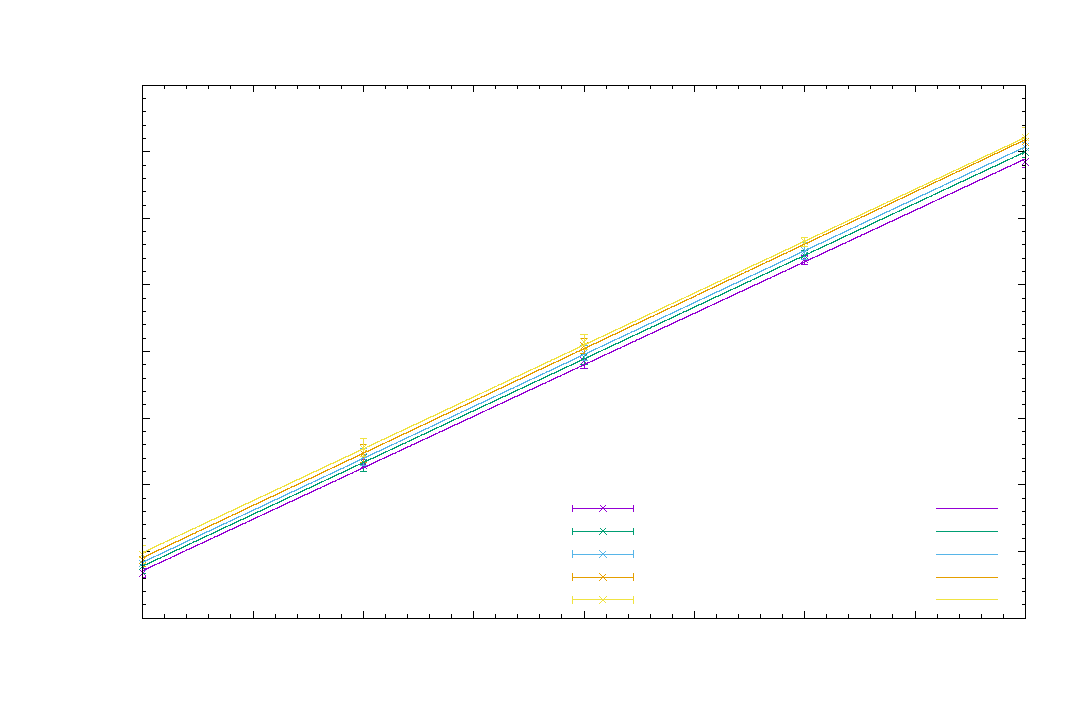
\includegraphics[width={504.00bp},height={324.00bp}]{tv4-l-plus}}%
    \gplfronttext
  \end{picture}%
\endgroup
}
	    \caption{Verlauf der Ringradien}
	    \vspace{-0.5em}
	    \label{fig:tv4-l-plus}
	\end{figure}
	\begin{center}
		\begin{tabular}{lrrrr}
			\toprule
			Strom $I/\si{\ampere}$ & $m/\si{\micro\meter\squared}$ & $c/\si{\micro\meter\squared}$ & $p_0$ & $\chi^2_\text{red}$ \\
			\midrule
	        \num{2.495(5)} & \num{7730,21963(7843301)} & \num{-4179,08793(26759715)} & \num{0,54062(3505)} & \num{0,47301} \\
	        \num{4.190(10)} & \num{7775,73625(2472955)} & \num{-3877,46605(9308847)} & \num{0,49866(1208)} & \num{0,03054} \\
	        \num{5.662(10)} & \num{7795,95244(2719018)} & \num{-3608,40828(10057227)} & \num{0,46286(1300)} & \num{0,03390} \\
	        \num{7.01(1)} & \num{7847,41240(7353670)} & \num{-3321,94377(27918566)} & \num{0,42332(3580)} & \num{0,24968} \\
	        \num{8.78(1)} & \num{7791,59699(6048853)} & \num{-2877,79824(21359518)} & \num{0,36935(2756)} & \num{0,08922} \\
			\bottomrule
		\end{tabular}
	\end{center}
	Die kleine $\chi^2_\text{red}$'s zeigt eine gute Kurveanpassung.  


